% Options for packages loaded elsewhere
% Options for packages loaded elsewhere
\PassOptionsToPackage{unicode}{hyperref}
\PassOptionsToPackage{hyphens}{url}
\PassOptionsToPackage{dvipsnames,svgnames,x11names}{xcolor}
%
\documentclass[
  12pt,
  oneside]{book}
\usepackage{xcolor}
\usepackage[top=30mm,bottom=30mm,left=25mm,right=20mm,headheight=15mm,footskip=33pt]{geometry}
\usepackage{amsmath,amssymb}
\setcounter{secnumdepth}{5}
\usepackage{iftex}
\ifPDFTeX
  \usepackage[T1]{fontenc}
  \usepackage[utf8]{inputenc}
  \usepackage{textcomp} % provide euro and other symbols
\else % if luatex or xetex
  \usepackage{unicode-math} % this also loads fontspec
  \defaultfontfeatures{Scale=MatchLowercase}
  \defaultfontfeatures[\rmfamily]{Ligatures=TeX,Scale=1}
\fi
\usepackage{lmodern}
\ifPDFTeX\else
  % xetex/luatex font selection
\fi
% Use upquote if available, for straight quotes in verbatim environments
\IfFileExists{upquote.sty}{\usepackage{upquote}}{}
\IfFileExists{microtype.sty}{% use microtype if available
  \usepackage[]{microtype}
  \UseMicrotypeSet[protrusion]{basicmath} % disable protrusion for tt fonts
}{}
\usepackage{setspace}
\makeatletter
\@ifundefined{KOMAClassName}{% if non-KOMA class
  \IfFileExists{parskip.sty}{%
    \usepackage{parskip}
  }{% else
    \setlength{\parindent}{0pt}
    \setlength{\parskip}{6pt plus 2pt minus 1pt}}
}{% if KOMA class
  \KOMAoptions{parskip=half}}
\makeatother
% Make \paragraph and \subparagraph free-standing
\makeatletter
\ifx\paragraph\undefined\else
  \let\oldparagraph\paragraph
  \renewcommand{\paragraph}{
    \@ifstar
      \xxxParagraphStar
      \xxxParagraphNoStar
  }
  \newcommand{\xxxParagraphStar}[1]{\oldparagraph*{#1}\mbox{}}
  \newcommand{\xxxParagraphNoStar}[1]{\oldparagraph{#1}\mbox{}}
\fi
\ifx\subparagraph\undefined\else
  \let\oldsubparagraph\subparagraph
  \renewcommand{\subparagraph}{
    \@ifstar
      \xxxSubParagraphStar
      \xxxSubParagraphNoStar
  }
  \newcommand{\xxxSubParagraphStar}[1]{\oldsubparagraph*{#1}\mbox{}}
  \newcommand{\xxxSubParagraphNoStar}[1]{\oldsubparagraph{#1}\mbox{}}
\fi
\makeatother


\usepackage{longtable,booktabs,array}
\newcounter{none} % for unnumbered tables
\usepackage{calc} % for calculating minipage widths
% Correct order of tables after \paragraph or \subparagraph
\usepackage{etoolbox}
\makeatletter
\patchcmd\longtable{\par}{\if@noskipsec\mbox{}\fi\par}{}{}
\makeatother
% Allow footnotes in longtable head/foot
\IfFileExists{footnotehyper.sty}{\usepackage{footnotehyper}}{\usepackage{footnote}}
\makesavenoteenv{longtable}
\usepackage{graphicx}
\makeatletter
\newsavebox\pandoc@box
\newcommand*\pandocbounded[1]{% scales image to fit in text height/width
  \sbox\pandoc@box{#1}%
  \Gscale@div\@tempa{\textheight}{\dimexpr\ht\pandoc@box+\dp\pandoc@box\relax}%
  \Gscale@div\@tempb{\linewidth}{\wd\pandoc@box}%
  \ifdim\@tempb\p@<\@tempa\p@\let\@tempa\@tempb\fi% select the smaller of both
  \ifdim\@tempa\p@<\p@\scalebox{\@tempa}{\usebox\pandoc@box}%
  \else\usebox{\pandoc@box}%
  \fi%
}
% Set default figure placement to htbp
\def\fps@figure{htbp}
\makeatother





\setlength{\emergencystretch}{3em} % prevent overfull lines

\providecommand{\tightlist}{%
  \setlength{\itemsep}{0pt}\setlength{\parskip}{0pt}}



 


\usepackage{Archivo}
%\usepackage[sc]{mathpazo}

\usepackage[T1]{fontenc}
\usepackage{xcolor}
\usepackage[pages=some]{background}
\usepackage{setspace}
\usepackage[table]{xcolor}
\usepackage{tabularx}
\usepackage[Bjornstrup]{fncychap}
\usepackage{multirow}

% Colors Techtraplastice
\definecolor{Naranja}{HTML}{F69223}
\definecolor{Celeste}{HTML}{3299CC}
\definecolor{Verde}{HTML}{98C601}
\definecolor{Neutro}{HTML}{5E6F75}
\definecolor{Neutro_claro}{HTML}{F1F1F1}

\definecolor{Verde_osc}{RGB}{47,93,80}


% Headers
\usepackage{fancyhdr}
\pagestyle{fancy}          

\fancyhead{}
\fancyfoot{}

\fancyhead[L]{
\includegraphics[height=10mm]{assets/images/logo-TTPCE.png}}
\fancyhead[C]{ }
\fancyhead[R]{\thepage}

\fancyfoot[L]{
\includegraphics[height=8mm]{assets/images/footer-00.png}}
\fancyfoot[C]{}
\fancyfoot[R]{
\includegraphics[height=8mm]{assets/images/EU.png}}



\renewcommand{\headrulewidth}{1pt}
\renewcommand{\headruleskip}{1mm}



\usepackage{pdfpages}
\usepackage{wrapfig}
\usepackage{pgfgantt}
\usepackage{academicons}

\usepackage{worldflags}

% Command
\newcommand{\techtra}{\emph{TechTraPlastiCE }}

\usepackage{tabu}

% \usepackage{sectsty}
% \sectionfont{\scshape}
\makeatletter
\@ifpackageloaded{caption}{}{\usepackage{caption}}
\AtBeginDocument{%
\ifdefined\contentsname
  \renewcommand*\contentsname{Table of contents}
\else
  \newcommand\contentsname{Table of contents}
\fi
\ifdefined\listfigurename
  \renewcommand*\listfigurename{List of Figures}
\else
  \newcommand\listfigurename{List of Figures}
\fi
\ifdefined\listtablename
  \renewcommand*\listtablename{List of Tables}
\else
  \newcommand\listtablename{List of Tables}
\fi
\ifdefined\figurename
  \renewcommand*\figurename{Figure}
\else
  \newcommand\figurename{Figure}
\fi
\ifdefined\tablename
  \renewcommand*\tablename{Table}
\else
  \newcommand\tablename{Table}
\fi
}
\@ifpackageloaded{float}{}{\usepackage{float}}
\floatstyle{ruled}
\@ifundefined{c@chapter}{\newfloat{codelisting}{h}{lop}}{\newfloat{codelisting}{h}{lop}[chapter]}
\floatname{codelisting}{Listing}
\newcommand*\listoflistings{\listof{codelisting}{List of Listings}}
\makeatother
\makeatletter
\makeatother
\makeatletter
\@ifpackageloaded{caption}{}{\usepackage{caption}}
\@ifpackageloaded{subcaption}{}{\usepackage{subcaption}}
\makeatother
\usepackage{bookmark}
\IfFileExists{xurl.sty}{\usepackage{xurl}}{} % add URL line breaks if available
\urlstyle{same}
% fallback for those not using the hyperref driver hyperxmp:
\makeatletter
\@ifundefined{xmpquote}{\newcommand{\xmpquote}[1]{#1}}{}
\makeatother
\hypersetup{
  pdftitle={D5.3 Project Website and Social Media accounts},
  pdfauthor={Lic. Marian Lenchours Pezzano ~; Mg. Marcos del Bello},
  colorlinks=true,
  linkcolor={Celeste},
  filecolor={Maroon},
  citecolor={Blue},
  urlcolor={Naranja},
  pdfcreator={LaTeX via pandoc}}


\title{D5.3 Project Website and Social Media accounts}
\author{Lic. Marian Lenchours Pezzano ~ \and Mg. Marcos del Bello}
\date{November 25, 2026}
\begin{document}
  \begin{frontmatter}
  \begin{titlepage}
  % Inspiration: https://nmfs-opensci.github.io/quarto_titlepages_v1/02-titlepages.html
  % This is a combination of Pandoc templating and LaTeX
  % Pandoc templating https://pandoc.org/MANUAL.html#templates
  % See the README for help



  \backgroundsetup{
    scale=1.0,
    angle=0,
    opacity=0.90,
    contents={
      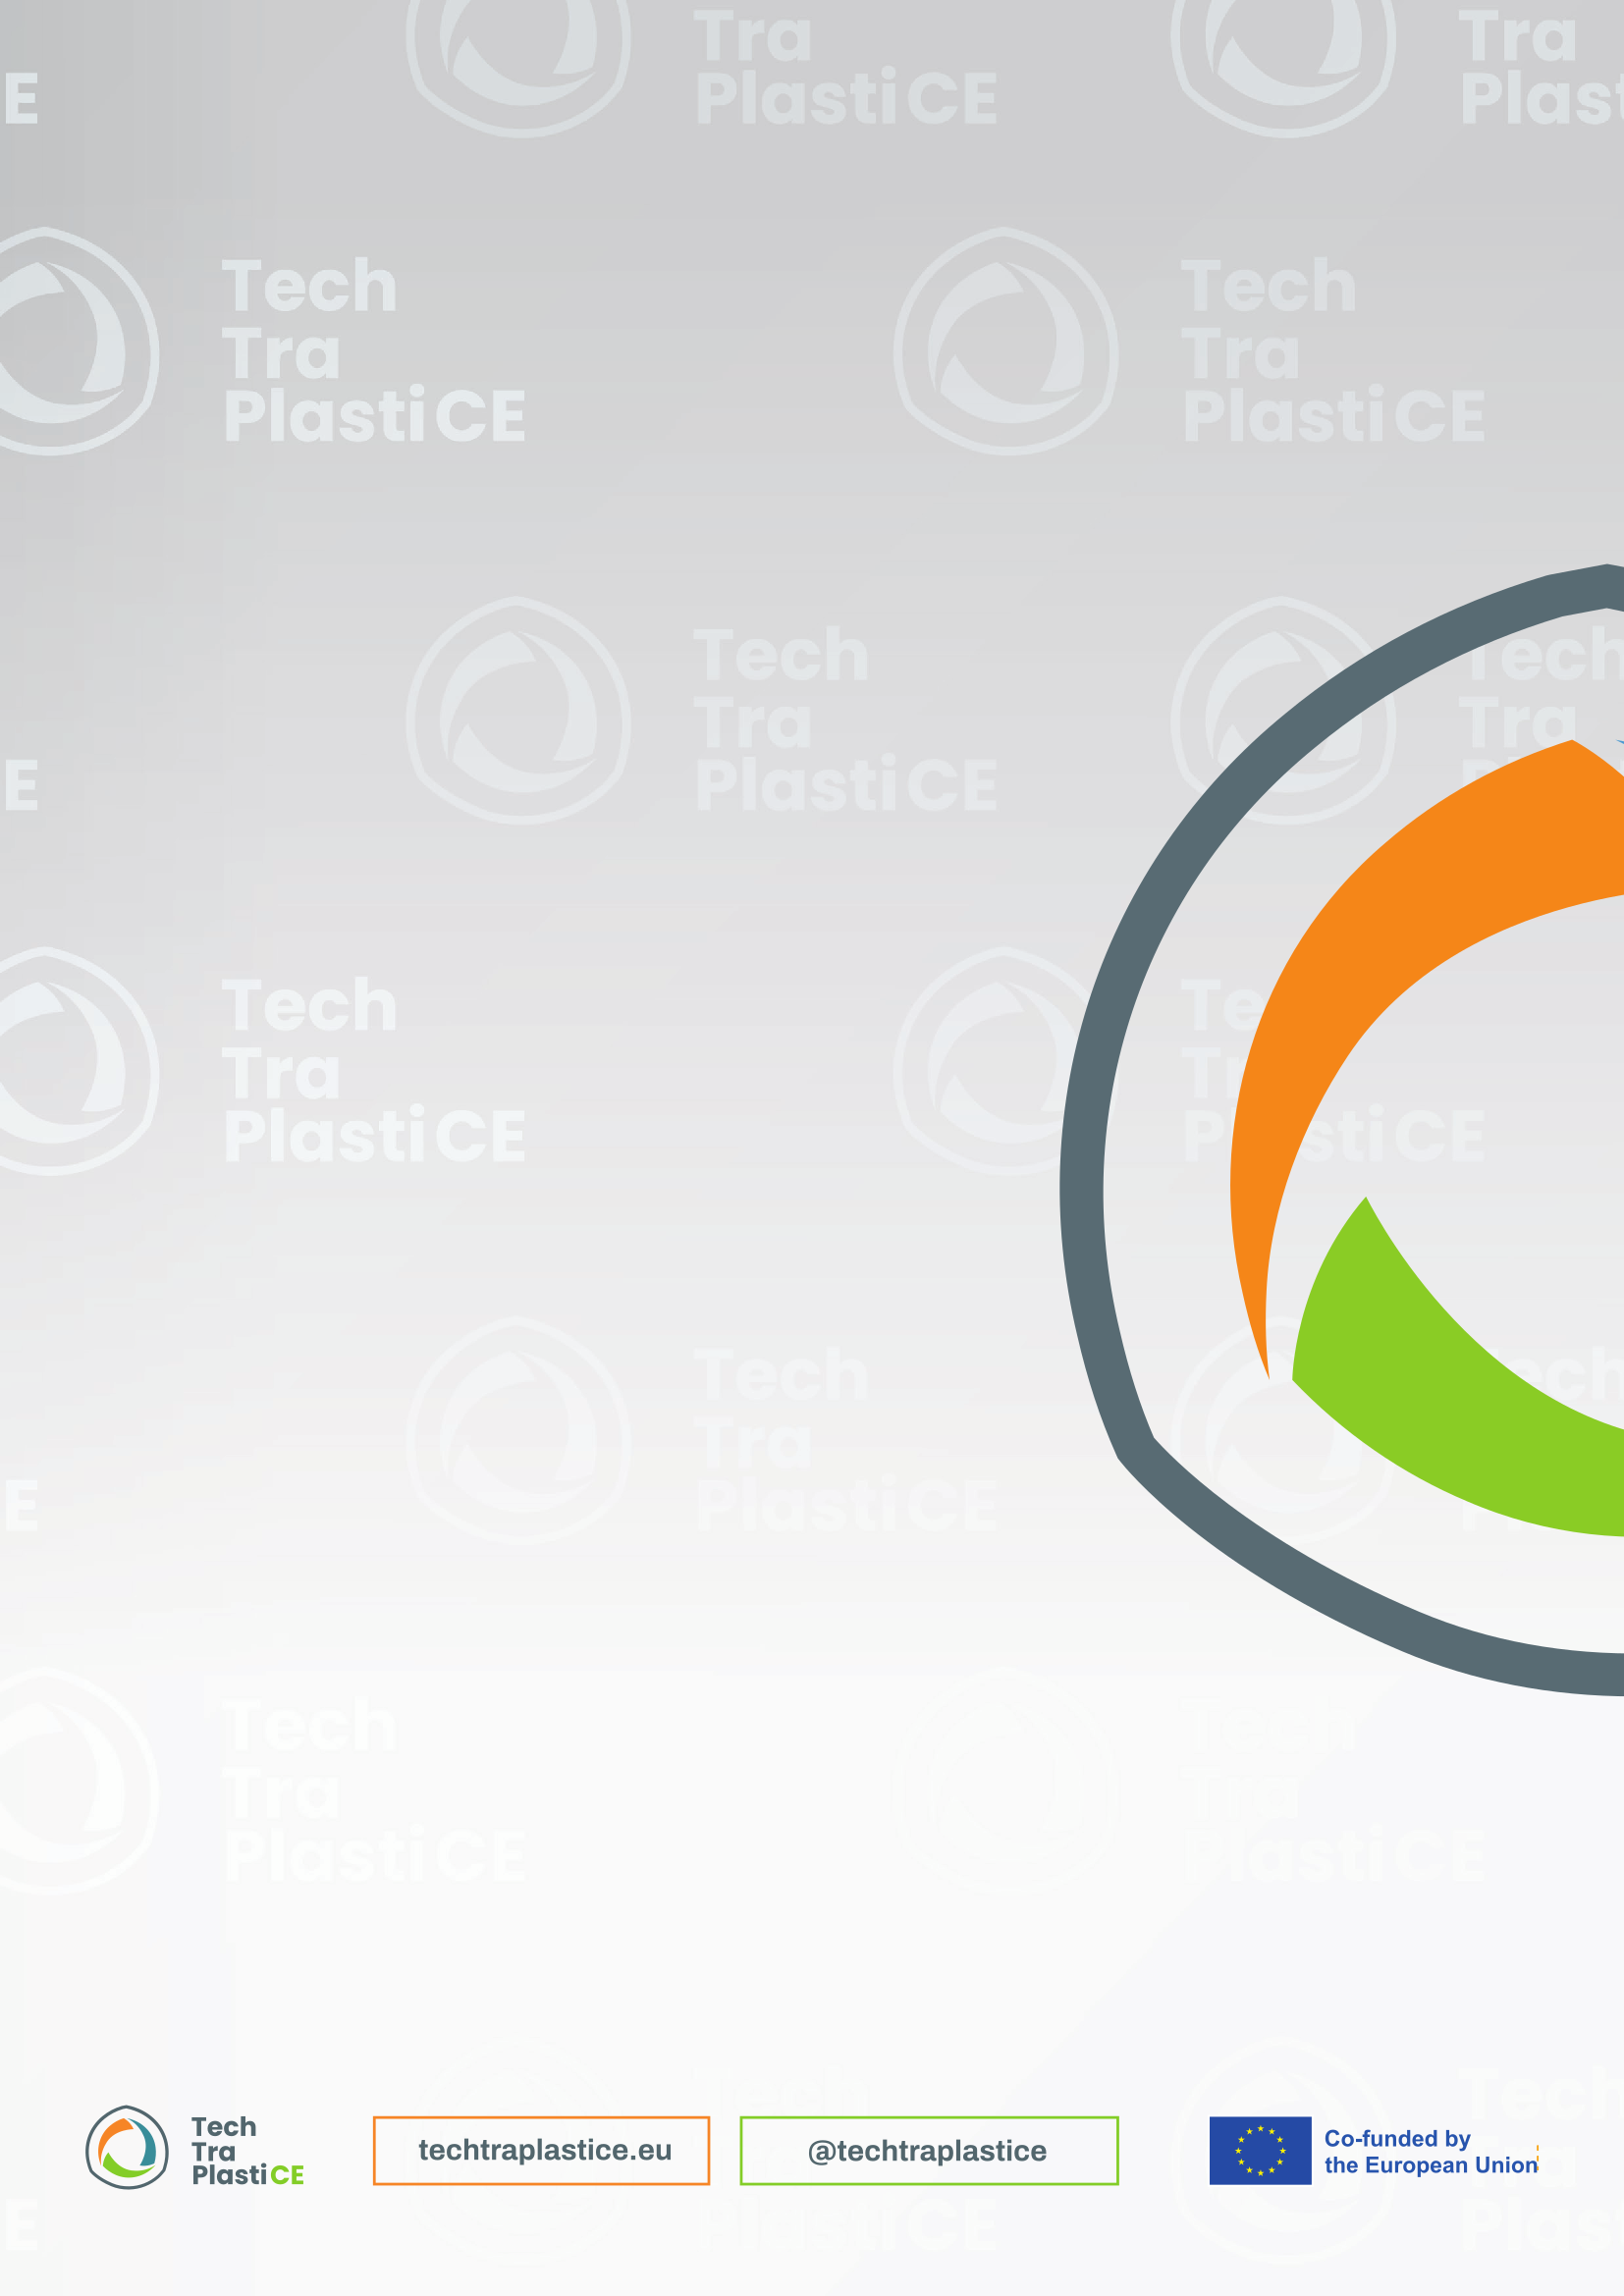
\includegraphics{assets/Portada.png}}
      }

  \BgThispage


  \begin{minipage}[b][0.78\textheight][s]{0.65\textwidth}

    \raggedright
    % Title and subtitle
    
    \vfill

    \begin{spacing}{2.2}
      {\color{Naranja}\Huge\bfseries{D5.3 Project Website and Social
  Media accounts}} \\[1\baselineskip] 
    \end{spacing}
    
    \begin{spacing}{1.2}
    {\color{Neutro} \Large\textit{WP5 -- Dissemination and
  Communication}}\\[1\baselineskip]
    
    {\Large \color{Neutro} 
    Strengthening University Tech Transfer Capabilities to Support Circular Economy 
    Value Chains for Plastics in Latin America -
    \textsc{\centering\bfseries TechTraPlastiCE} }\\[2\baselineskip]

    
    \end{spacing}

    {\color{Neutro} \Large\textit{November 25, 2026}}
    
    \vfill
  \end{minipage}		

  \vfill

  {\scriptsize
    \color{Neutro}
    This project has been funded with the support of Erasmus +.  
    The contents are the responsibility of the author(s). 
    The Commission cannot be held responsible for any use which may be made of the information contained therein. 
    Project No. 101179564 
    }


  \newpage



  \thispagestyle{plain}
  \begin{tabu} to \linewidth {X[1.3,l]  | X[1,l] X[1,l]}
    \toprule
    \multirow{5}{*}{ 
\includegraphics[height=20mm]{assets/images/logo-TTPCE.png}} &  \textbf{Work Package} : & WP5  \\ \cmidrule{2-3}
      & \textbf{Project Number} : & 101179564  \\ \cmidrule{2-3}
      &  \textbf{Type of document}:  & Deliverable   \\ \cmidrule{2-3}
      & \textbf{Due Delivery Date}:    & June
  30/2025     \\ \cmidrule{2-3}
      & \textbf{Actual Delivery Date}:    & November 25, 2026       \\ 
    \bottomrule
  \end{tabu}

  \vfill


  \begin{tabu} to \linewidth {X[1,l]  | X[3.5,l]}
    \toprule
    \textbf{Title} : & D5.3 Project Website and Social Media
  accounts  \\ \cmidrule{2-2}
    \textbf{Work Package} : & WP5 -- Dissemination and
  Communication  \\ \cmidrule{2-2}
    \textbf{Description} : & The creation of the website and social
  media accounts will be produced by the beginning of the project and
  available for all partners and targets.  \\ \cmidrule{2-2}
    \textbf{Responsible} : & Universidad Nacional de Río
  Negro  \\ \cmidrule{2-2}
    \textbf{Author(s)} : &  
     
          Lic. Marian Lenchours Pezzano ~
          
          Mg. Marcos del Bello
           \\ \cmidrule{2-2}
    \textbf{Project Call} : & ERASMUS-EDU-2024-CBHE (Capacity building in the field of higher education)  \\ \cmidrule{2-2}
    \textbf{Dissemination Level} : & Confidential\\   
  \bottomrule
  \end{tabu}



  \vfill


  \begin{tabular}{ >{\raggedright\arraybackslash}p{3cm}| p{2cm} p{3cm} p{7cm} }
    \toprule
    \textbf{Version}: & \multicolumn{3}{l}{1.3} \\ \midrule
    \textbf{Contributors}  & Versions    & Dates       & Revision Description \\ \midrule
    WP5 Leader  & 1.0    & June 26/2025  & First version  \\ 
    Coordinator  & 1.1    & July 02/2025  & Improvement of graphs  \\ 
    Coordinator  & 1.2    & July 08/2025  & Validation to submit  \\ 
    \bottomrule
\end{tabular}  


    
    
    \vfill
    
    {\scriptsize\centering\color{lightgray} 
    
    Disclaimer
    
    This document is provided <<as is>> with no warranties whatsoever, 
    including any warranty or merchantability, non-infringement, fitness for any particular 
    purpose, or any warranty otherwise arising out of any proposal, specification or sample.  
    
    No license, express or implied, by estoppels or otherwise, to any intellectual 
    property rights are granted herein. 
    The members of the project TechTraPlastiCE do not accept any liability for actions or 
    omissions of TechTraPlastiCE members or third parties and disclaim any obligation 
    to enforce the use of this document. 
    
    This document reflects only the authors' view and the Commission is not responsible 
    for any use that may be made of the information it contains.  
    This document is subject to change without notice. 
    
    }
    \normalsize
    
    
    
      \end{titlepage}
  \end{frontmatter}

\renewcommand*\contentsname{Contents}
{
\setcounter{tocdepth}{2}
\tableofcontents
}
\listoffigures

\setstretch{1.2}
\mainmatter
\chapter{Executive Summary}\label{executive-summary}

Deliverable \textbf{D5.3 -- Project Website and Social Media Accounts}
presents the development, deployment, and coordination of
TechTraPlastiCE's digital communication ecosystem, led by the
\emph{Universidad Nacional de Río Negro (UNRN)} under \textbf{Work
Package 5 -- Communication and Dissemination}.\\
This deliverable outlines the establishment of the project's official
website --- \url{https://techtraplastice.eu} --- and its associated
social media channels on \textbf{LinkedIn}, \textbf{X (formerly
Twitter)}, and \textbf{YouTube}, which collectively ensure visibility,
engagement, and accessibility of the project's activities and outputs.

The website serves as the \textbf{primary communication platform} for
the consortium, providing updated information about project objectives,
news, events, and results. It is designed to deliver clear, accessible,
and bilingual content (English and Spanish) targeting diverse audiences,
from higher education stakeholders and researchers to enterprises and
policy actors in the plastic value chain. The site's structure ---
comprising \emph{Home, Project, Partners, News, Agenda,} and
\emph{Contact} sections --- supports intuitive navigation and
transparent communication of the project's scope and achievements.

A monthly content calendar and standardized templates coordinate partner
contributions to the website's \textbf{News} and \textbf{Agenda}
sections, ensuring timely and coherent dissemination.\\
All key project deliverables will be made publicly available upon
completion, in accordance with the \textbf{EACEA's principle of
knowledge sharing}.

To extend outreach beyond the website, a coordinated social media
strategy integrates \textbf{LinkedIn, X, and YouTube} as complementary
dissemination tools. These platforms are used to highlight project
milestones, promote events, share multimedia materials, and redirect
audiences toward the main website.\\
Partners are encouraged to actively engage by sharing, reposting, and
commenting on content to amplify visibility through their institutional
and professional networks.

The dissemination strategy also emphasizes \textbf{multi-level
engagement}: - At the \textbf{local level}, within Higher Education
Institutions (HEIs), to build internal capacity and awareness; - At the
\textbf{national level}, to connect with enterprises, chambers of
commerce, and associations linked to the plastic value chain; and - At
the \textbf{international level}, to contribute to scientific and policy
discussions on the circular economy transition.

The \textbf{WP5 leader} maintains a monitoring database to track partner
contributions, ensuring balanced participation and systematic evaluation
of communication impact.\\
User experience (UX) analysis confirms that the website's design ---
minimalistic, responsive, and professionally branded --- effectively
reflects the project's academic and technological nature. It combines
visual clarity, functional usability, and a consistent identity aligned
with the European Commission's visibility requirements.

Overall, Deliverable D5.3 demonstrates that the TechTraPlastiCE website
and social media channels effectively support the project's mission to
\textbf{promote knowledge exchange, visibility, and stakeholder
engagement} throughout its lifecycle.

\chapter{Introduction}\label{introduction}

Effective communication and dissemination are key enablers of the
TechTraPlastiCE mission, which aims to strengthen the applied research
and innovation capacities of Higher Education Institutions (HEIs) to
become relevant actors in the circular economy transition within the
plastic value chain in the Latin American context.

In this regard, The \emph{Universidad Nacional de Río Negro (UNRN)}
leads Work Package 5 (WP5) -- Dissemination and Communication, which
plays a strategic role in ensuring that the project's objectives,
activities, and results are effectively communicated to a broad range of
stakeholders at local, national, and international levels. With the
support and coordination of the Université de Lorraine (UL -- P1), the
entire TechTraPlastiCE consortium contributes actively to maximizing
visibility and impact throughout the project's lifecycle.

WP5 encompasses a comprehensive set of deliverables designed to
implement the project's dissemination and communication strategy:

\begin{itemize}
\tightlist
\item
  D5.1 -- Digital Communication Strategy ,
\item
  D5.2 -- Branding Toolkit and Training Plan ,
\item
  D5.3 -- \textbf{Project Website and Social Media Accounts},
\item
  D5.4 -- Open Digital Repository , and
\item
  D5.5 -- Final Conference and Results Summary .
\end{itemize}

This document presents \textbf{Deliverable D5.3 -- Project Website and
Social Media Accounts}, developed under \textbf{Work Package 5 (WP5) --
Communication and Dissemination}, led by the \emph{Universidad Nacional
de Río Negro (UNRN)}.\\
The deliverable focuses on the \textbf{design, structure, and
deployment} of the official TechTraPlastiCE website
(\href{techtraplastice.eu}{https://techtraplastice.eu/}) and associated
social media channels
(\href{https://www.linkedin.com/company/techtraplastice/}{@techtraplastice
on LinkedIn}, \href{https://x.com/techtraplastice}{X}, and
\href{https://www.youtube.com/@TechTraPlastiCE}{Youtube}), which
together form the project's digital communication ecosystem. These
digital tools function as the main communication and interaction
channels for the project, providing a central space where external
stakeholders can access official updates, activities, and results.

In alignment with the \emph{Digital Strategy for Dissemination and
Exploitation (Deliverable D5.1)}, this deliverable supports the
project's overarching objective of \textbf{amplifying outreach and
engagement} through both dedicated and partner-led channels.\\
This includes leveraging additional networks such as \emph{Facebook} and
\emph{Instagram}, where the project may not maintain direct accounts but
can still ensure visibility through partners and associated initiatives.

The integrated communication and dissemination strategy described in
this deliverable is designed to:

\begin{itemize}
\tightlist
\item
  Foster engagement among stakeholders and target audiences;
\item
  Enhance the visibility of project results and activities; and
\item
  Ensure the \emph{long-term sustainability and accessibility} of
  TechTraPlastiCE outputs beyond the project's duration.
\end{itemize}

This document is structured in three major section. First, project
website launching and monitoring is detailed. Then, a focus wil be made
on the social media accounts.

\chapter{\texorpdfstring{TechTraPlastiCE Website launching and
Monitoring
--\href{https://techtraplastice.eu}{techtraplastice.eu/}--}{TechTraPlastiCE Website launching and Monitoring --techtraplastice.eu/--}}\label{techtraplastice-website-launching-and-monitoring-techtraplastice.eu}

TechTraPlastiCE aims to deliver the \emph{right message to the right
audience}. As highlighted in \emph{Deliverable D5.1 -- Digital Strategy
for Dissemination and Exploitation}, it is essential that all relevant
stakeholders are continuously informed through timely and updated
information on project activities, news, and events.

Therefore, the project website \url{https://techtraplastice.eu} (see
Figure Figure~\ref{fig-web}) serves as the \textbf{main communication
platform} for the TechTraPlastiCE consortium. It provides a clear and
accessible overview of the project's progress, achievements, and
outputs. The website is designed to be comprehensive, and regularly
updated, ensuring that information is relevant and understandable for a
broad public audience as well as for specific target groups.

\begin{figure}[H]

\centering{

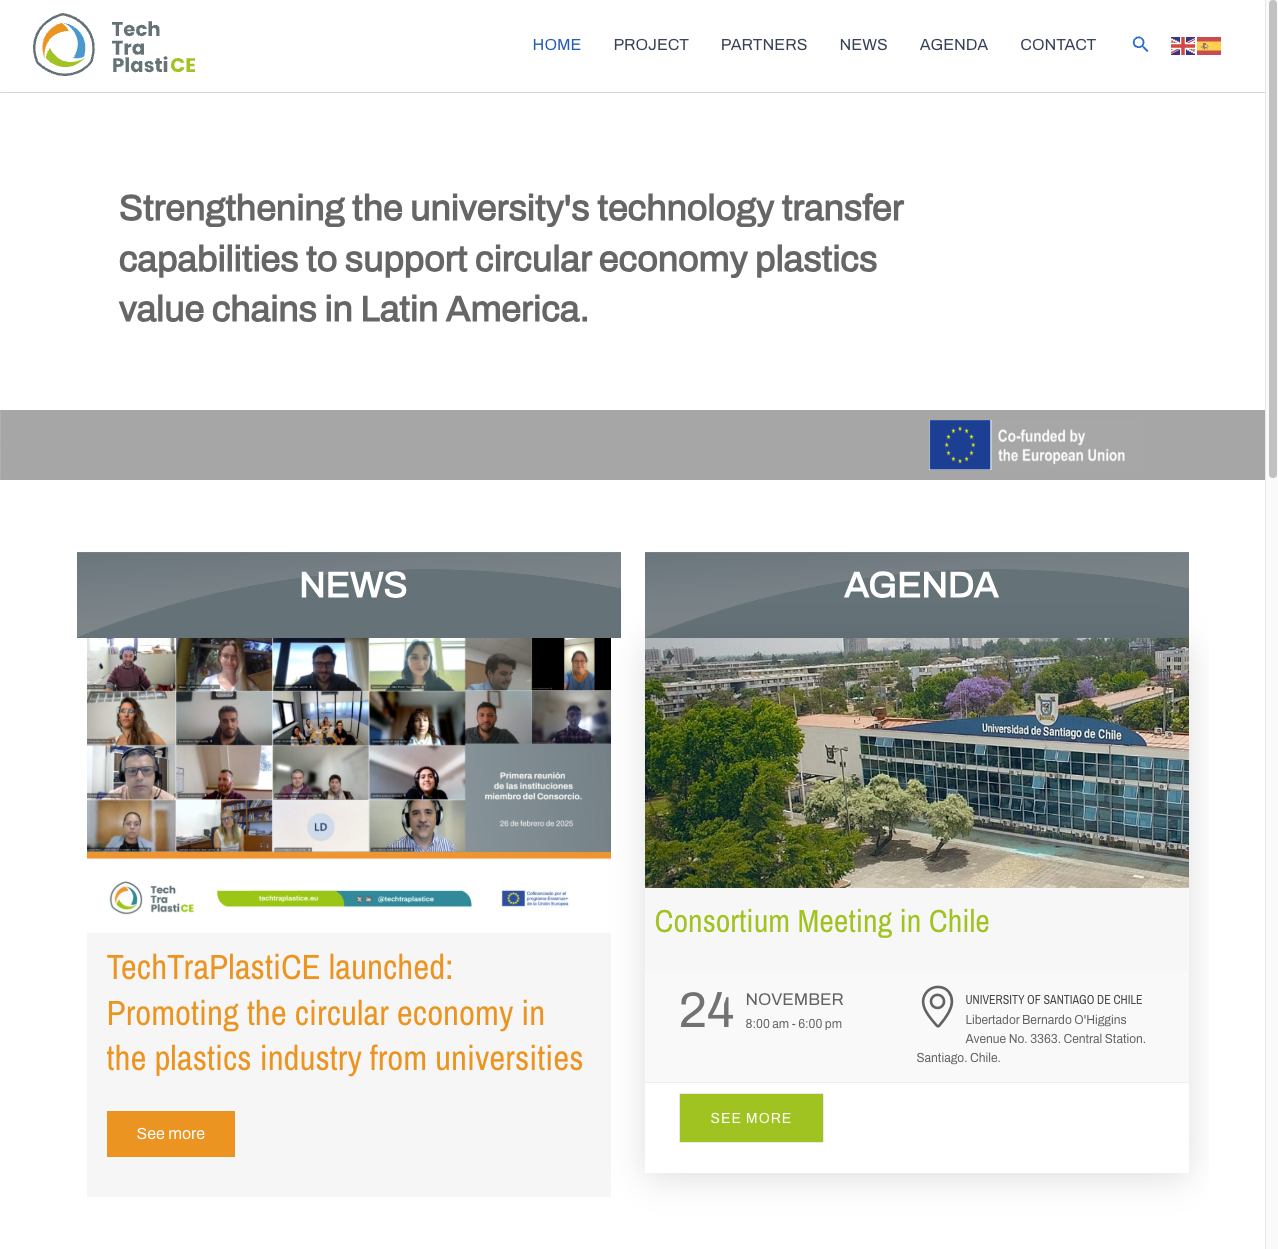
\includegraphics[width=0.7\linewidth,height=\textheight,keepaspectratio]{figures/5.3/website-00.png}

}

\caption{\label{fig-web}Project Website:
\url{https://techtraplastice.eu/}}

\end{figure}%

In addition, all project results will be promoted through the partners'
national and international networks, thereby maximizing impact and
ensuring wide outreach across sectors and regions.

\section{TechTraPlastiCE Website
Visibility}\label{techtraplastice-website-visibility}

All communication and dissemination actions are designed to direct
audiences to the official TechTraPlastiCE website for further
information and for contacting the project management team. To maximize
outreach, the website is also interconnected with each partner's
institutional communication channels, ensuring consistent visibility
across the consortium network.

To enhance visibility and reach a broader audience throughout the
project's implementation, the website is actively cross-linked with
other relevant institutional, national, and international platforms that
support the dissemination objectives of TechTraPlastiCE.

\begin{figure}[H]

\centering{

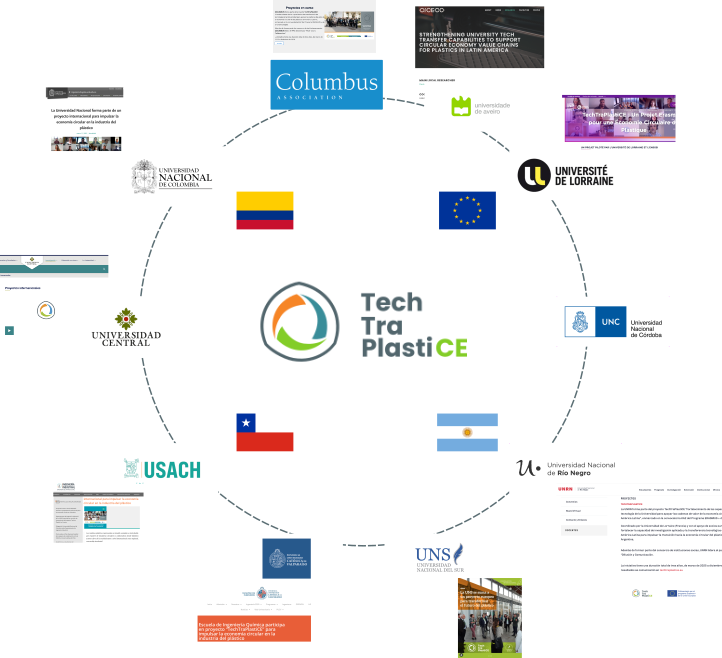
\includegraphics[width=0.7\linewidth,height=\textheight,keepaspectratio]{figures/5.3/Visibility.png}

}

\caption{\label{fig-web}TechTraPlastiCE Website visibility:
\url{https://techtraplastice.eu/}}

\end{figure}%

In this regard, each partner university or organization has a dedicated
webpage pointing to the official TechTraPlastiCE website, thereby
strengthening its online presence and ensuring coherence across partner
communications. The current list of partner webpages referencing
TechTraPlastiCE includes:

\begin{itemize}
\tightlist
\item
  \textbf{Université de Lorraine (France):}
  \href{https://ensgsi.univ-lorraine.fr/recherche-ensgsi/chaires-partenariales-et-grands-projets-ensgsi/techtraplastice-un-projet-erasmus-pour-une-economie-circulaire-du-plastique/}{TechTraPlastiCE
  -- un projet Erasmus+ pour une économie circulaire du plastique}
\item
  \textbf{Columbus Association:}
  \href{https://columbus-web.org/servicios/}{COLUMBUS forma parte del
  proyecto TechTraPlastiCE}
\item
  \textbf{Universidad Central de Colombia:}
  \href{https://www.ucentral.edu.co/investigacion/proyectos-internacionales}{Proyectos
  Internacionales -- Universidad Central}
\item
  \textbf{Universidad Nacional de Colombia:}
  \href{https://ingenieria.bogota.unal.edu.co/la-universidad-nacional-forma-parte-de-un-proyecto-internacional-para-impulsar-la-economia-circular-en-la-industria-del-plastico/}{La
  Universidad Nacional forma parte de un proyecto internacional para
  impulsar la economía circular en la industria del plástico}
\item
  \textbf{Universidad Nacional de Río Negro (UNRN):}
  \href{https://www.unrn.edu.ar/section/38/programas-y-redes.html}{Programas
  y Redes -- UNRN}
\item
  \textbf{Universidad Nacional del Sur (UNS):}
  \href{https://internacionalizacion.uns.edu.ar/techtraplastice/}{La
  Universidad Nacional del Sur se suma a un proyecto europeo para
  fortalecer la economía circular del plástico.}
\item
  \textbf{Pontifia Universidad Católica de Valparaiso (PUCV):}
  \href{https://www.ingenieria.pucv.cl/escuela-de-ingenieria-quimica-participa-en-proyecto-techtraplastice-para-impulsar-la-economia-circular-en-la-industria-del-plastico/}{Escuela
  de Ingeniería Química participa en proyecto ``TechTraPlastiCE''}
\item
  \textbf{Universidad de Santiago de Chile (USACH):}
  \href{https://www.ingenieriaindustrial-usach.cl/noticias/proyecto-erasmus-techtraplastice-avanza-en-propuestas-de-soluciones-para-la-economia-circular-en-colombia/}{Proyecto
  Erasmus TechTraPlastiCE avanza en propuestas de soluciones para la
  economía circular}
\end{itemize}

These institutional links significantly contribute to increasing the
visibility of TechTraPlastiCE, reinforcing its credibility, and
promoting engagement across the consortium's extended networks.

\section{Content creation and
dissemination}\label{content-creation-and-dissemination}

The TechTraPlastiCE website will be \emph{updated on a monthly basis} to
ensure that all information remains current and relevant. The WP5 leader
is responsible for designing, administering, and maintaining the
website, in close collaboration with all project partners.

To coordinate content production, a monthly dissemination calendar (see
Figure Figure~\ref{fig-calendar}) has been established. This calendar
defines the contributions expected from each partner for the
\textbf{News} and \textbf{Agenda} sections, thereby ensuring regular and
balanced updates across the consortium.

\begin{figure}[H]

\centering{

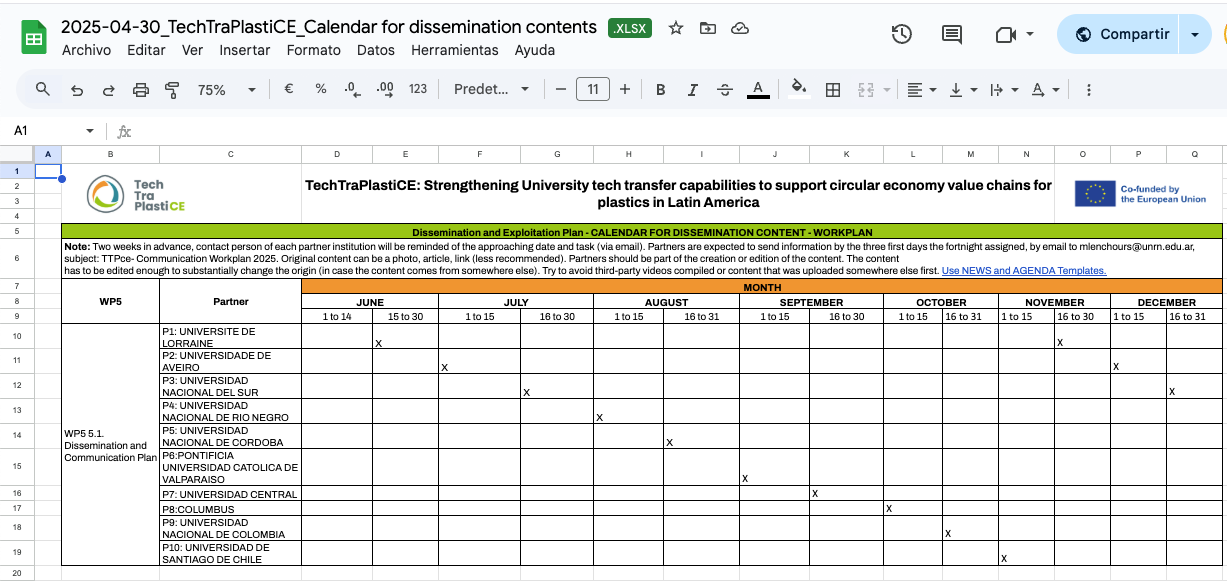
\includegraphics[width=0.9\linewidth,height=\textheight,keepaspectratio]{figures/5.3/Calendar.png}

}

\caption{\label{fig-calendar}Calendar for dissemination contents}

\end{figure}%

To facilitate the preparation of dissemination materials,
\textbf{standardized templates} have been provided to all partners (see
Section Section~\ref{sec-template}). These templates define the expected
content format, specify the required information fields, and outline the
\textbf{image format and usage rights} to ensure compliance with
copyright and communication guidelines.

\subsection{Multi-Level Dissemination and Partner
Engagement}\label{multi-level-dissemination-and-partner-engagement}

In line with the EACEA's principle of knowledge sharing, the most
significant project deliverables and outputs will be made publicly
available on the project website once finalized, ensuring open and easy
access to key results and resources.

As illustrated in Figure~\ref{fig-vis2}, the main objective is to enable
each partner institution to disseminate project outcomes at
\textbf{local}, \textbf{national}, and \textbf{international} levels,
according to their specific networks and outreach capacity.

\begin{figure}[H]

\centering{

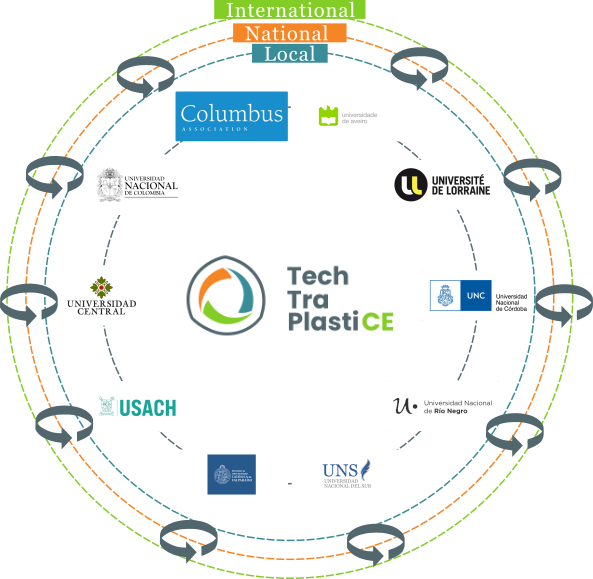
\includegraphics[width=0.4\linewidth,height=\textheight,keepaspectratio]{figures/5.3/Visibility-2.png}

}

\caption{\label{fig-vis2}Visibility}

\end{figure}%

\begin{itemize}
\item
  \textbf{Local level:} Refers to the internal audiences within each
  Higher Education Institution (HEIs) population --- including students,
  researchers, and academic staff.\\
  Dissemination at this level aims to identify and strengthen local
  competences within the HEIs, thereby enhancing their institutional
  capacity and expanding their educational and innovation portfolio in
  the field of circular economy.
\item
  \textbf{National level:} Encompasses outreach to enterprises, chambers
  of commerce, professional associations, and other relevant actors of
  the plastic value chain.\\
  Dissemination activities at this scale allow project results to reach
  stakeholders who can directly benefit from or contribute to the
  practical implementation of the project's outcomes.
\item
  \textbf{International level:} Involves participation in scientific
  conferences, publications, and academic collaborations that arise from
  the collective work of the consortium.\\
  Although TechTraPlastiCE is primarily a capacity-building project, it
  also contributes to the broader research agenda on the circular
  economy transition in the plastics sector, a topic of growing societal
  and scientific relevance.
\end{itemize}

To effectively coordinate these multi-level dissemination activities,
the WP5 leader maintains a monitoring database (see
Figure~\ref{fig-vis3}).\\
This tool allows for systematic tracking of the content generated and
shared by each partner, ensuring balanced contributions and identifying
opportunities to leverage each HEI's local and national networks for
maximum dissemination impact.

\begin{figure}[H]

\centering{

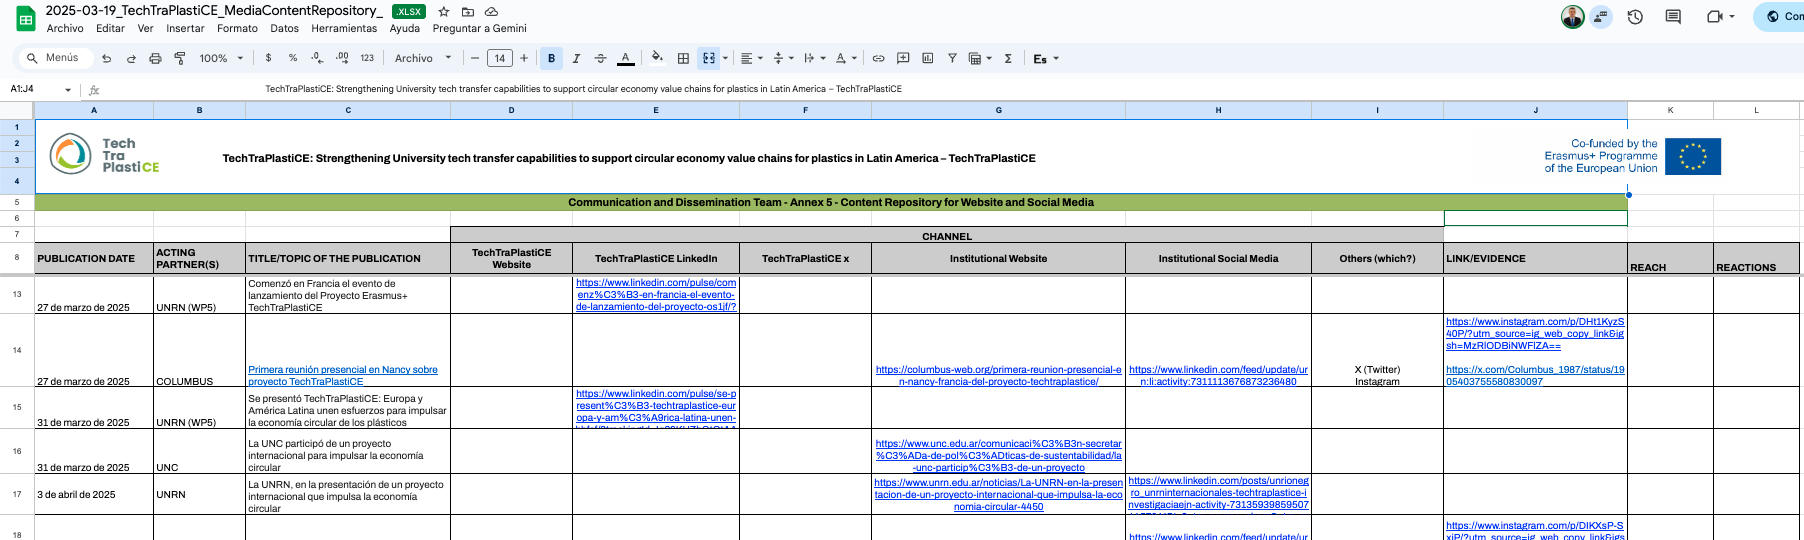
\includegraphics[width=1\linewidth,height=\textheight,keepaspectratio]{figures/5.3/Visibility-3.png}

}

\caption{\label{fig-vis3}Partner Dissemination Monitoring Database}

\end{figure}%

\section{Website tree structure and
components}\label{website-tree-structure-and-components}

A first version of the TechTraPlastiCE website was created in February
2025 for the kick off meeting. It was completed in June 2025 with all
sections and functionalities required for the initial stage of the
project. The final version of the project will be ready towards the end
of the project, with the section corresponding to the Open Digital
Repository (D5.4) where the results of this initiative

\begin{figure}[H]

\centering{

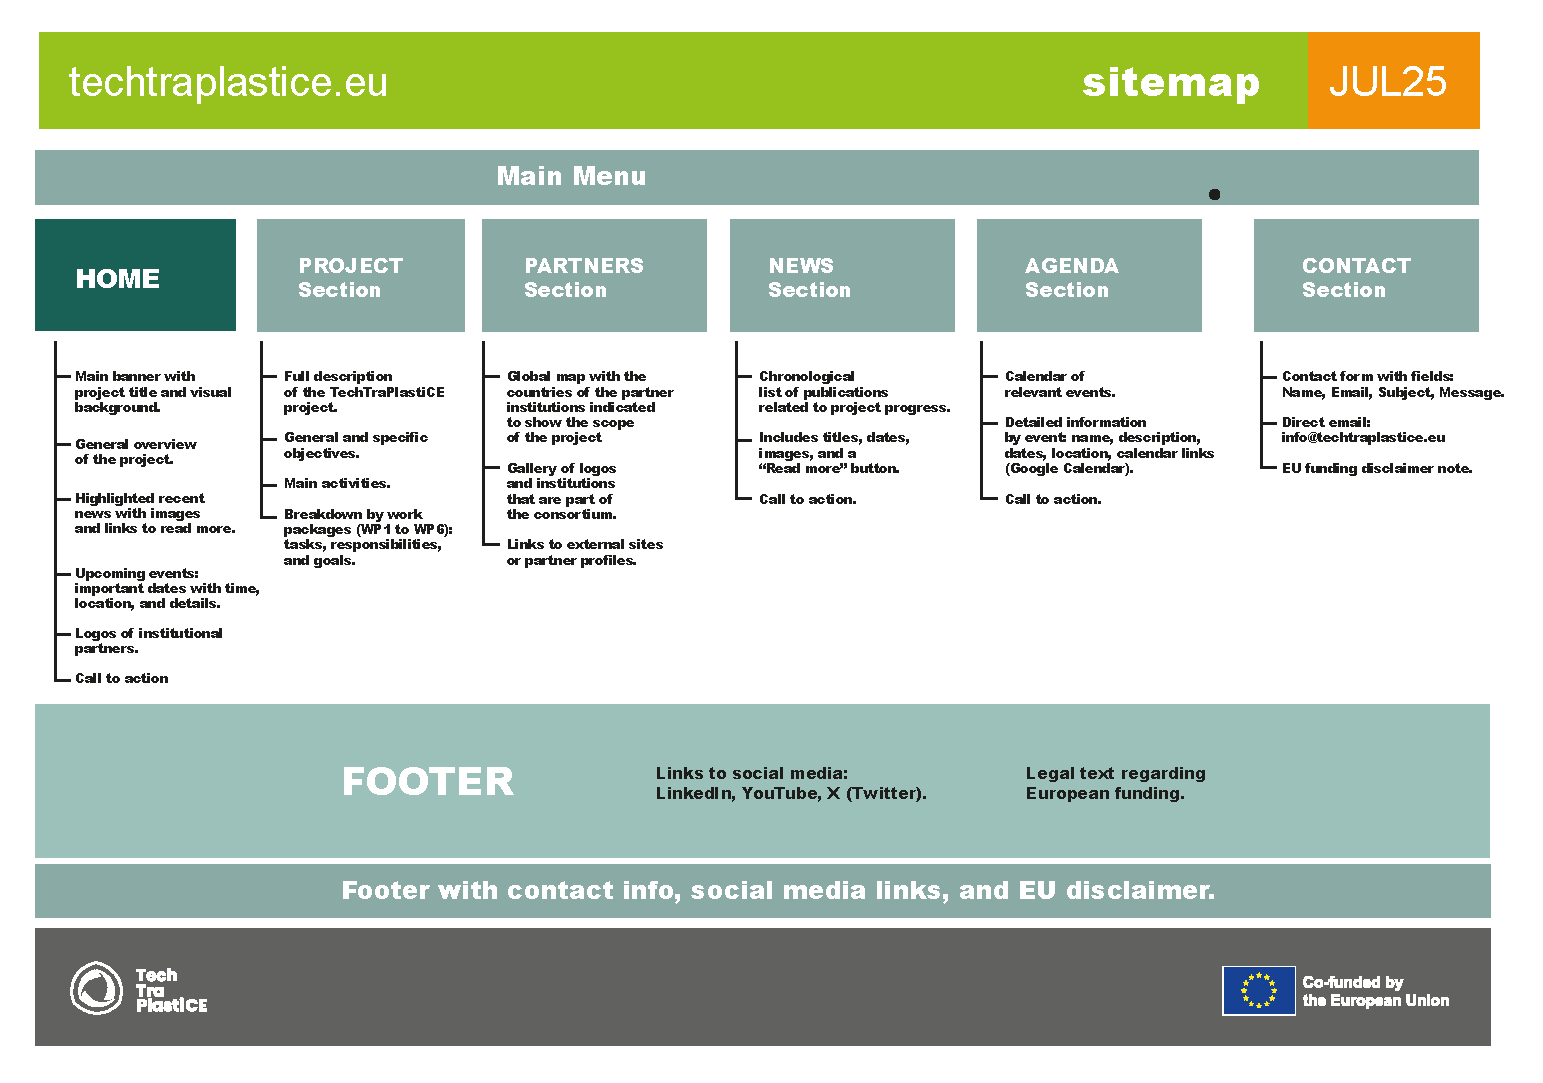
\includegraphics[width=0.9\linewidth,height=\textheight,keepaspectratio]{figures/5.3/Arbol.pdf}

}

\caption{\label{fig-home}TechTraPlastiCE Website structuration}

\end{figure}%

The TechTraPlastiCE project website is organized into a clear and
accessible structure that communicates the scope, goals, and progress of
the initiative. The layout is divided into several core sections: Home,
Project, Partners, News, Agenda, and Contact, with each fulfilling a
specific communication role.

The \emph{HOME} (Figure~\ref{fig-home}) section serves as the landing
page and includes a banner showcasing the project title and an engaging
visual background to capture the visitor's attention. This area sets the
tone for the site, inviting users to explore further. The section
highlights recent news items, with images and links to full articles,
showcasing ongoing progress, events, and developments within the
project. Also, upcoming activities are presented under ``Agenda'',
listing key dates, event titles, locations, and short descriptions to
engage users and promote participation. Below, visitors are introduced
to the full description of the TechTraPlastiCE consortium.

At the \emph{Project} section (Figure \ref{fig-project}), the main goal
is to outline the project's description, objective and results related
to plastic circularity and sustainable innovation. The main activities
are detailed here, providing an overview of how the project intends to
achieve its goals.

\begin{wrapfigure}{l}{0.65\textwidth}
  \begin{center}
    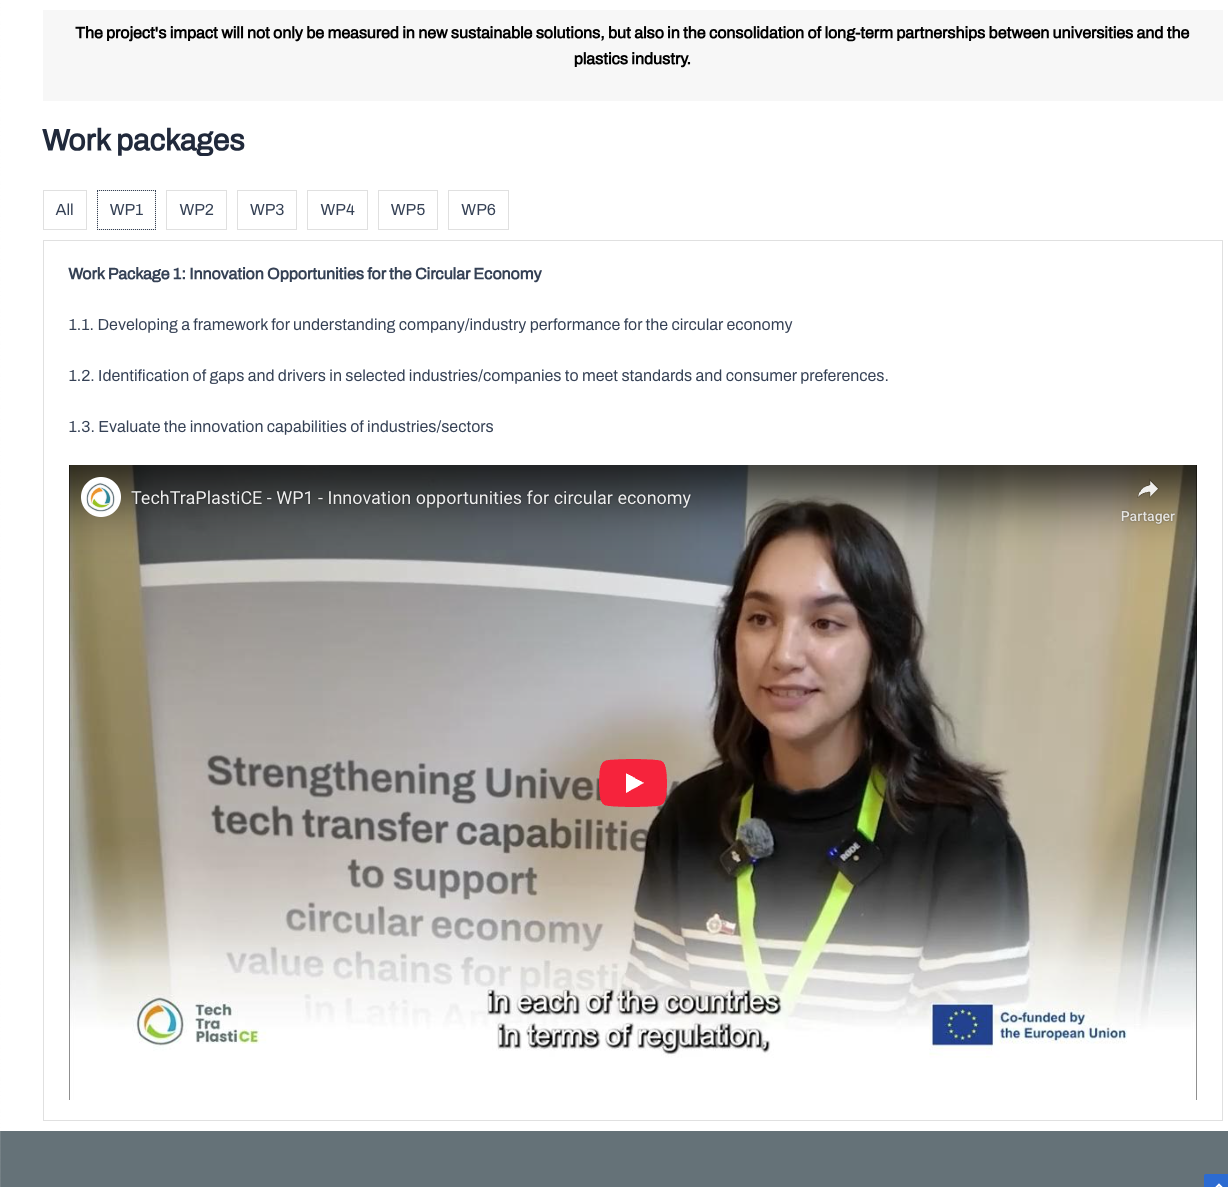
\includegraphics[width=0.60\textwidth]{figures/5.3/website-01.png}
  \end{center}
  \caption{Project section of TechTraPlastiCE website \label{fig-project}}
\end{wrapfigure}

A significant feature of this section is the breakdown by work packages
(WP1 to WP6). Each work package is presented with a description of its
tasks, roles of participating institutions, and specific goals. This
breakdown helps to demonstrate the project's strategic planning and
operational roadmap.

On the other hand, the \emph{PARTNERS} section emphasizes the
collaborative nature of TechTraPlastiCE. It features a global map
indicating the countries where partner institutions are based, visually
conveying the project's international scope. A gallery of logos displays
the institutions involved, and each is linked to external websites or
profiles, providing visitors with further information about the
consortium.

The \emph{NEWS} section (Figure~\ref{fig-news}) compiles all
project-related publications in a chronological list. Each entry
includes the title, date, a featured image, and a ``Read more'' button,
allowing users to follow project milestones and access detailed updates.
This section helps demonstrate transparency, dissemination of results,
and community outreach.

\begin{figure}[H]

\centering{

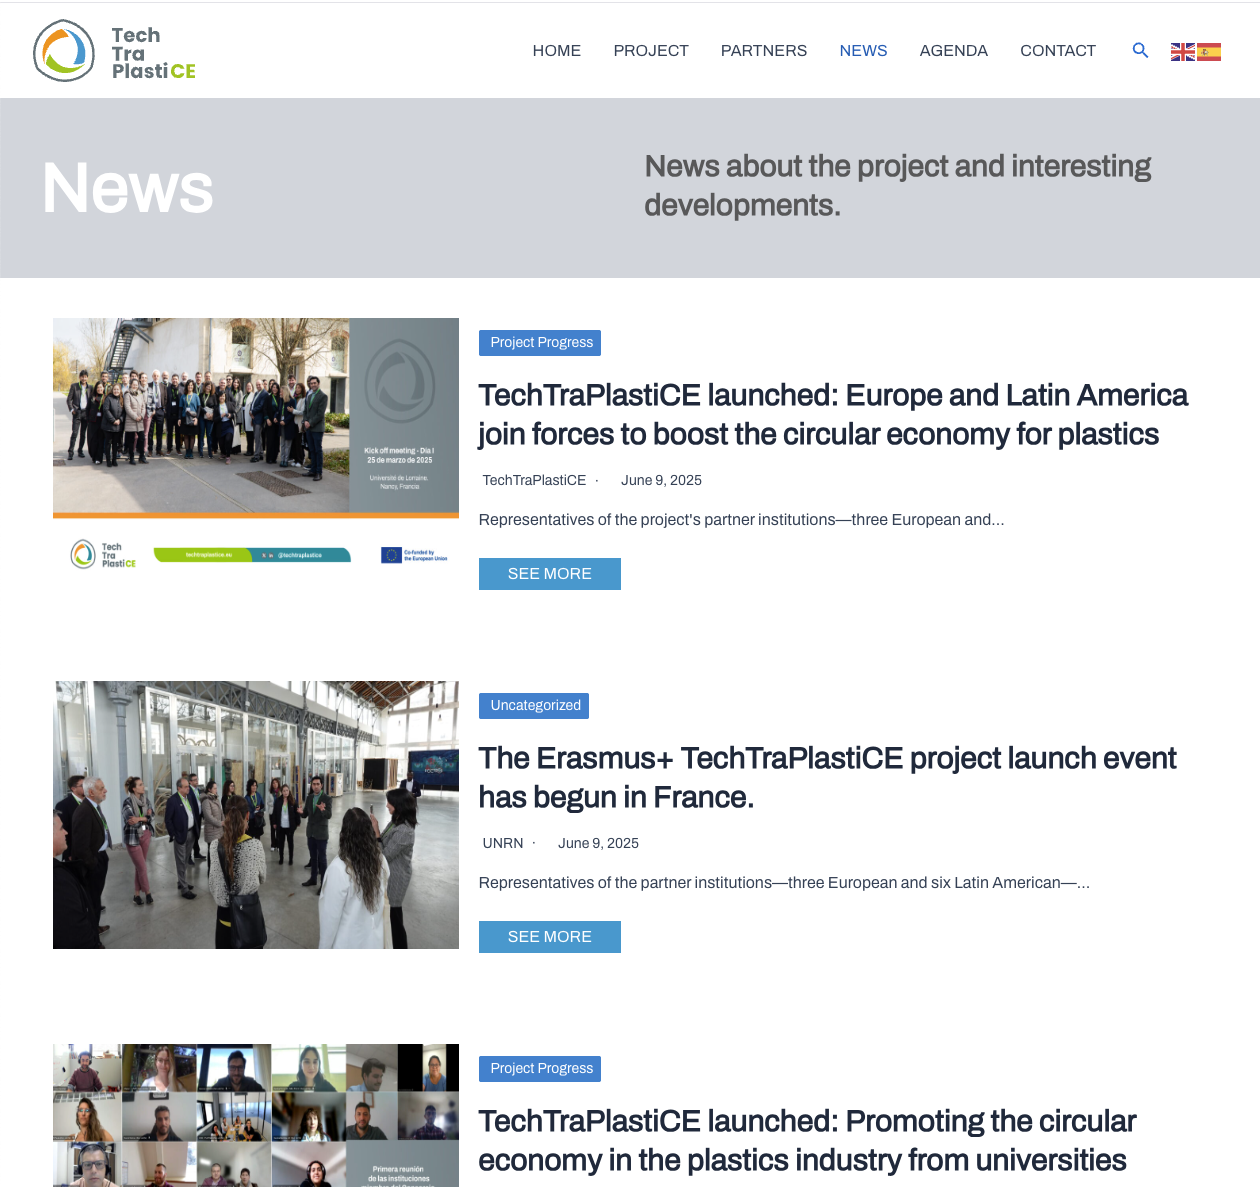
\includegraphics[width=0.6\linewidth,height=\textheight,keepaspectratio]{figures/5.3/website-02.png}

}

\caption{\label{fig-news}TechTraPlastiCE Website structure}

\end{figure}%

In the \emph{AGENDA} section (Figure~\ref{fig-agenda}), users can find a
calendar of relevant events. Each listing provides comprehensive details
such as the event name, description, date, location, and direct links to
add the event to personal calendars (e.g., Google Calendar). This
encourages active participation from stakeholders and the general
public.

\begin{figure}[H]

\centering{

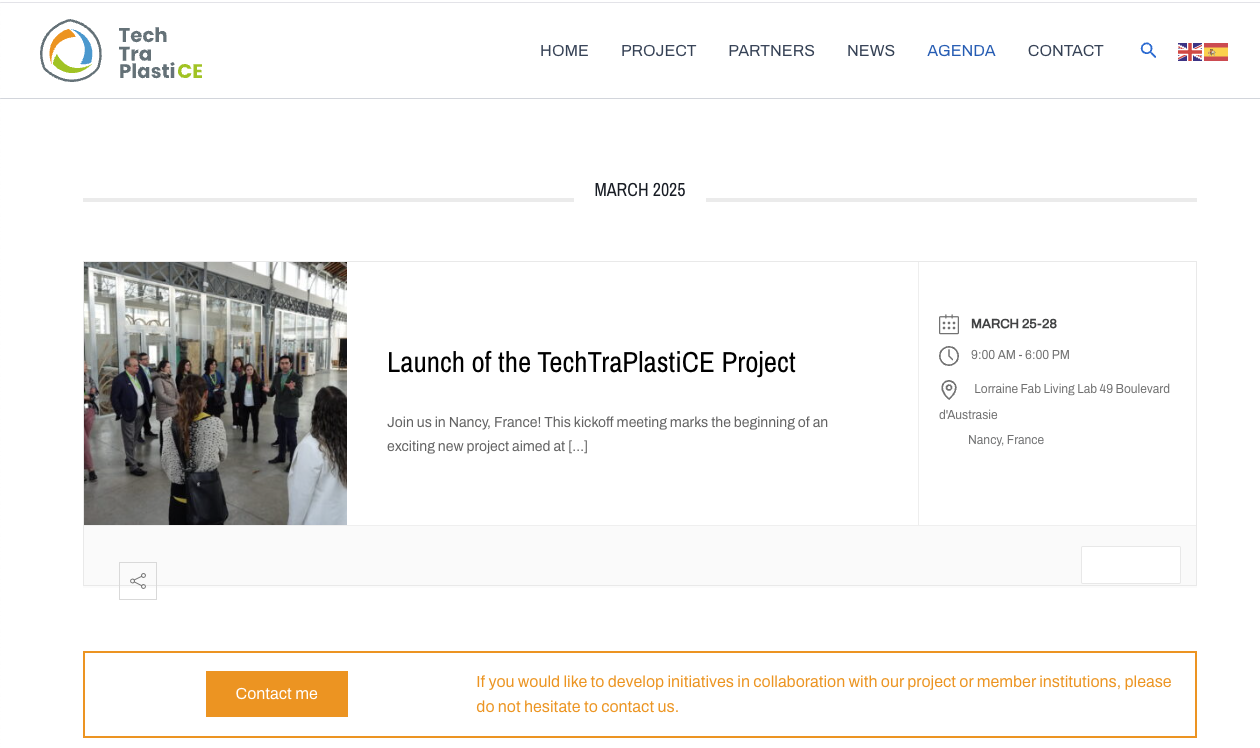
\includegraphics[width=0.6\linewidth,height=\textheight,keepaspectratio]{figures/5.3/website-03.png}

}

\caption{\label{fig-agenda}Agenda}

\end{figure}%

The footer across the site contains essential elements such as legal
text, EU funding disclaimers, and quick access to social media channels.
Overall, the TechTraPlastiCE website tree reflects a well-organized,
user-friendly interface that supports communication, transparency, and
collaboration within a major European research initiative.

\section{Stakeholder Engagement and Contact
Mechanisms}\label{stakeholder-engagement-and-contact-mechanisms}

All communication actions are designed to direct audiences toward the
project website, which serves as the central hub for further information
and for contacting the project management team.

One of the innovative features of TechTraPlastiCE is the early and
continuous engagement of HEIs with the local ecosystem of the plastic
value chain, initiated already in \emph{WP1 Innovation Opportunities for
Circular Economy} .\\
This strategy of TechTraPlastiCE aims to ignite a close interaction
since the beginning between academia, industry, and society, ensuring
that project activities are aligned with real-world challenges and
opportunities.

\begin{figure}[H]

\centering{

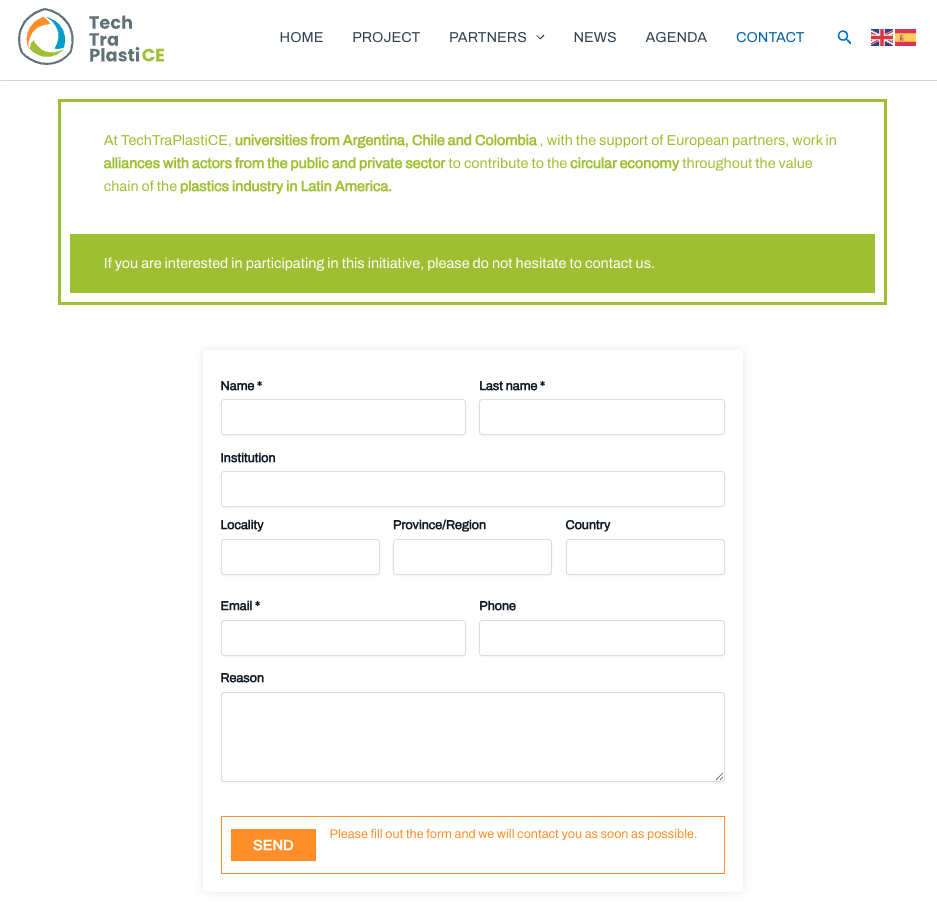
\includegraphics[width=0.7\linewidth,height=\textheight,keepaspectratio]{figures/5.3/Engagement.png}

}

\caption{\label{fig-engagement}External stakeholder contact to
TechTraPlastiCE consortium}

\end{figure}%

To facilitate this engagement, the website includes a dedicated contact
form (see Figure~\ref{fig-engagement}) that enables \textbf{external
stakeholders} to reach the TechTraPlastiCE consortium directly.
\textbf{This is very important in order to identify the enterprises that
want to be part of the project in Colombia, Chile and Argentina
contexts}.

The \emph{CONTACT} section includes a contact form where users can
submit inquiries by filling in their name, email, subject, and message.
Additionally, a direct email address
\href{mailto:info@techtraplastice.eu}{\nolinkurl{info@techtraplastice.eu}}
is provided for more direct communication. This feature supports
potential collaboration and knowledge exchange throughout the project's
lifetime. This contact mechanism also plays a key role in the
exploitation phase, enabling interested stakeholders to access
information and tools that support the transfer and adoption of project
results beyond its completion.

At the end of the project, all final outputs and dissemination materials
will be made publicly available through the Open Educational Resources
(OERs) platform, as are going to be detailed in Deliverables D5.4 and
D5.5.

\section{User Experience Report
(UX/UI)}\label{user-experience-report-uxui}

The TechTraPlastiCE website features a clean and professional design
that aligns with the academic and technological nature of the project as
illustrated in Figure~\ref{fig-ux}.

Its visual identity has been developed to reflect the standards commonly
associated with European research initiatives, prioritizing clarity,
reliability, and institutional presence. The overall aesthetic avoids
unnecessary ornamentation or visual clutter, favoring a minimalist and
structured layout that enhances user experience. The site's design
serves not only as a visual representation of the project's credibility
but also as a practical tool for communication and dissemination. This
thoughtful approach ensures that the content is easily accessible to a
wide audience, including researchers, partners, policymakers, and the
general public. Every element on the website contributes to a sense of
coherence and professionalism, reinforcing the project's role within the
broader European research and innovation landscape.

\begin{figure}[H]

\centering{

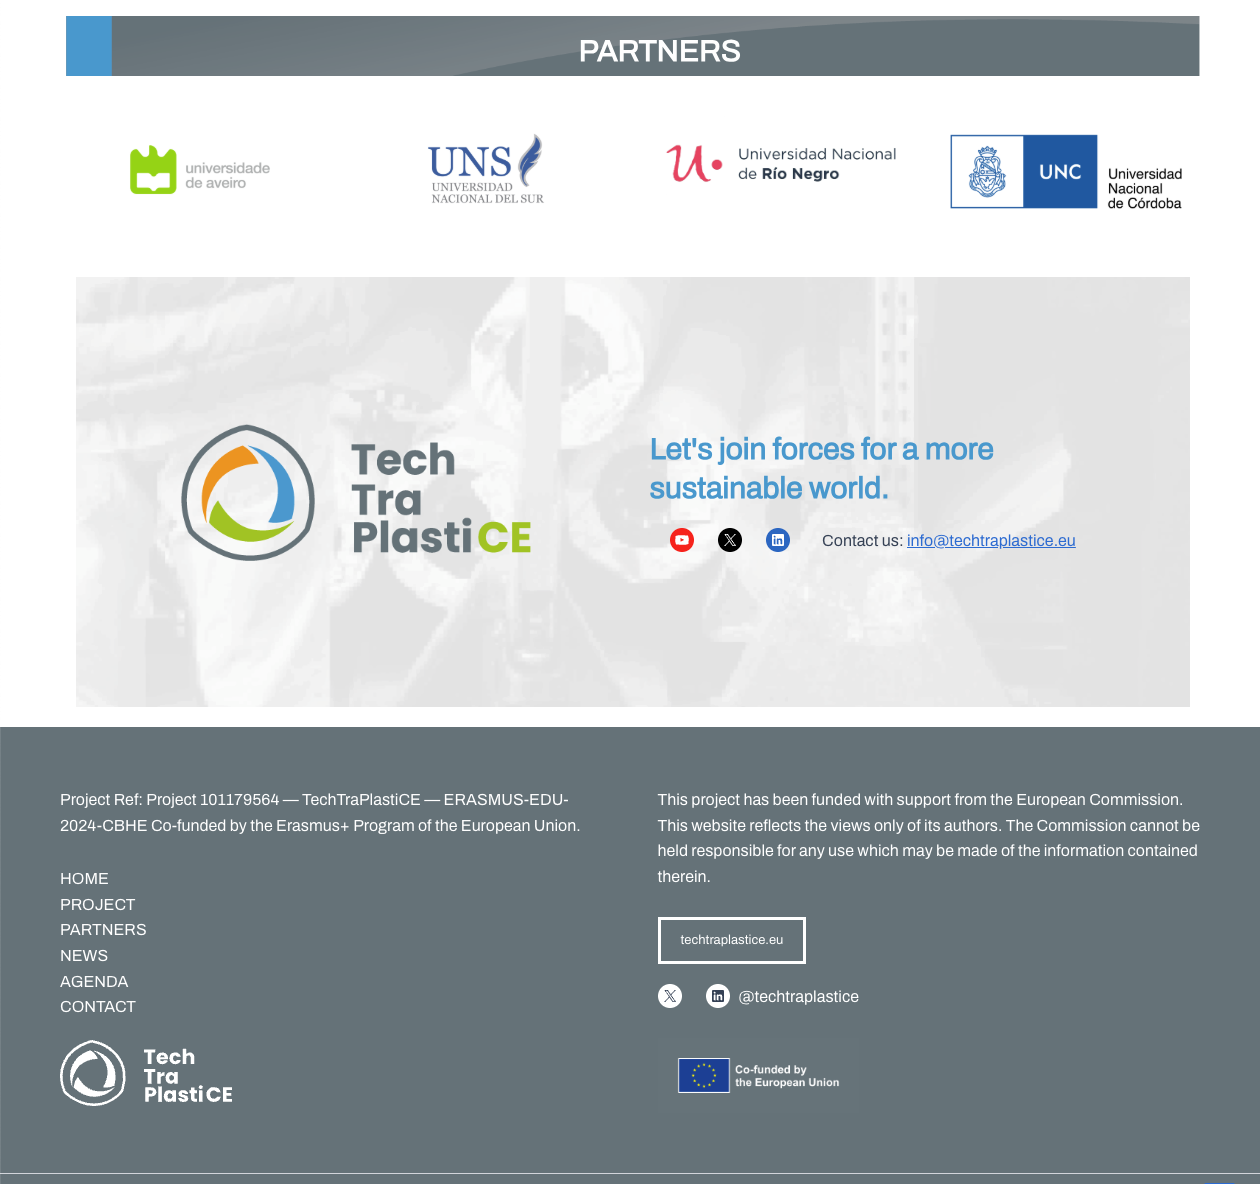
\includegraphics[width=0.8\linewidth,height=\textheight,keepaspectratio]{figures/5.3/ux.png}

}

\caption{\label{fig-ux}TechTraPlastiCE legibility}

\end{figure}%

A key component of the site's identity is its color palette, defined in
Deliverable D5.1, which is dominated by shades of blue and gray. These
colors were chosen not only for aesthetic appeal but also for the
psychological associations they carry. Blue tones evoke a sense of
trust, innovation, and intelligence---values strongly aligned with
scientific and technological progress---while gray adds a sense of
balance, neutrality, and professionalism. This controlled use of color
helps maintain visual harmony across the site, supporting its formal
tone without being monotonous. The palette is applied consistently
throughout all sections, from banners and buttons to text highlights and
backgrounds, ensuring a unified appearance. The result is a visual
identity that is both modern and serious, which reflects the strategic
goals of the project and enhances its credibility among stakeholders in
the European research community.

Typography and layout are also carefully considered to promote clarity
and legibility. The font choices are clean and sans-serif, ensuring that
all text remains easy to read across different devices and screen sizes.
There is no overuse of bold styles, decorative elements, or distracting
graphic effects, which reinforces the project's commitment to
\emph{functional design}. Content is organized into well-defined blocks,
each with ample white space, making the site feel open and easy to
navigate. Images and icons are used moderately and strategically to
support the information, not overwhelm it.

This minimalistic and structured approach contributes to an intuitive
user experience, helping users find relevant content quickly and without
distraction. Overall, the website's visual and structural design
reflects a balance between aesthetic restraint and practical usability,
in line with the professional and research-driven focus of
TechTraPlastiCE.

\subsection{Usability and Access to
Information}\label{usability-and-access-to-information}

The TechTraPlastiCE website intends a well-thought-out structure and
user-friendly design, particularly in terms of navigation and content
accessibility in \textbf{English and Spanish} given the international
context as presented in Figure~\ref{fig-consortium}. A clear top menu
provides direct links to the main sections---Home, Project, Partners,
News, and Agenda---ensuring users can easily find key information.

\begin{figure}[H]

\centering{

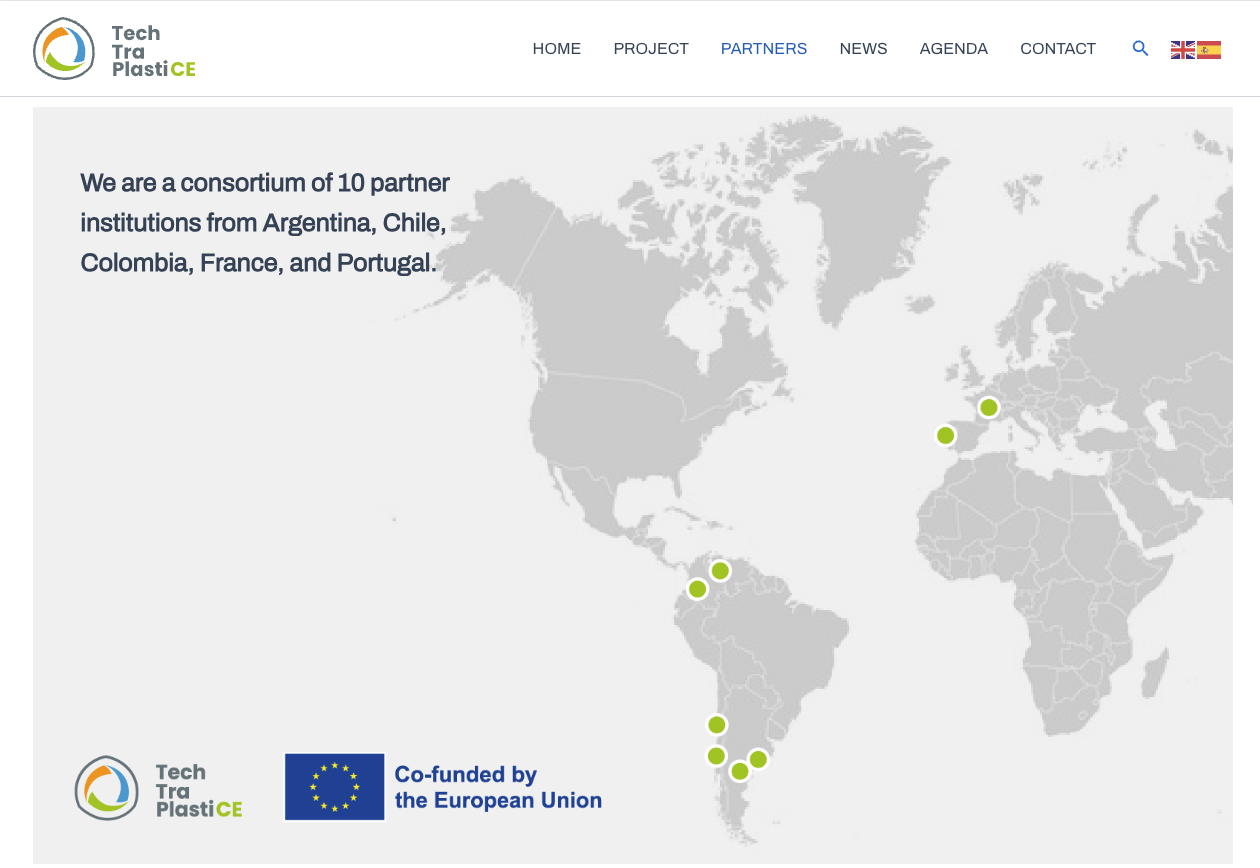
\includegraphics[width=0.8\linewidth,height=\textheight,keepaspectratio]{figures/5.3/consortium.png}

}

\caption{\label{fig-consortium}TechTraPlastiCE in Spanish and English as
international project}

\end{figure}%

The site is responsive and functions well on mobile devices, although
certain areas, such as the news modules, could benefit from improved
formatting for smaller screens. Content is logically organized, with
each section featuring concise titles, short descriptive paragraphs, and
calls to action like ``see more'' to guide user interaction.

On the homepage, news and events are prominently displayed, drawing
attention to the latest updates and project milestones. Additionally,
the site includes several useful features, such as calendar integration
for events, external links to partner institutions and social media
platforms, and visible contact information in the footer.

These elements collectively contribute to a functional, accessible, and
informative user experience.

\subsection{Observations and Opportunities for
Improvement}\label{observations-and-opportunities-for-improvement}

The WP5 leader, with the support of the project's Communication Team,
will enhance the visual dimension of the website by increasing the use
of images, infographics, and visual storytelling elements to better
communicate the project's objectives and results to non-technical
audiences, particularly within the Project section.

Furthermore, the website will evolve dynamically in response to emerging
communication and dissemination needs, ensuring that its content remains
relevant and engaging throughout the project's implementation. These
improvements will be progressively defined and implemented in
coordination with the development of each Work Package, ensuring
alignment between project activities and communication outputs.

\chapter{Social Media of TechTraplastiCE: LinkedIn, Youtube and
X}\label{social-media-of-techtraplastice-linkedin-youtube-and-x}

Figure~\ref{fig-social} lists the social media accounts that will be
used as communication channels. LinkedIn \footnote{Linkedin :
  \url{https://www.linkedin.com/company/techtraplastice/}.} and X
\footnote{X : \url{https://x.com/techtraplastice}.} (@techtraplastice)
were defined as the most suitable social media network for the
TechTraPlastiCE Project to engage with a broader audience and to
disseminate its results. A YouTube \footnote{YouTube :
  \href{https://www.youtube.com/@TechTraPlastiCE}{https://www.youtube.com/@TechTraPlastiCE}.}
channel of the project was also created to host all the audiovisual
material of the project, which will be also linked to the website,
newsletters and other social networks, as appropriate.

\begin{figure}[H]

\begin{minipage}[t]{0.32\linewidth}

\centering{

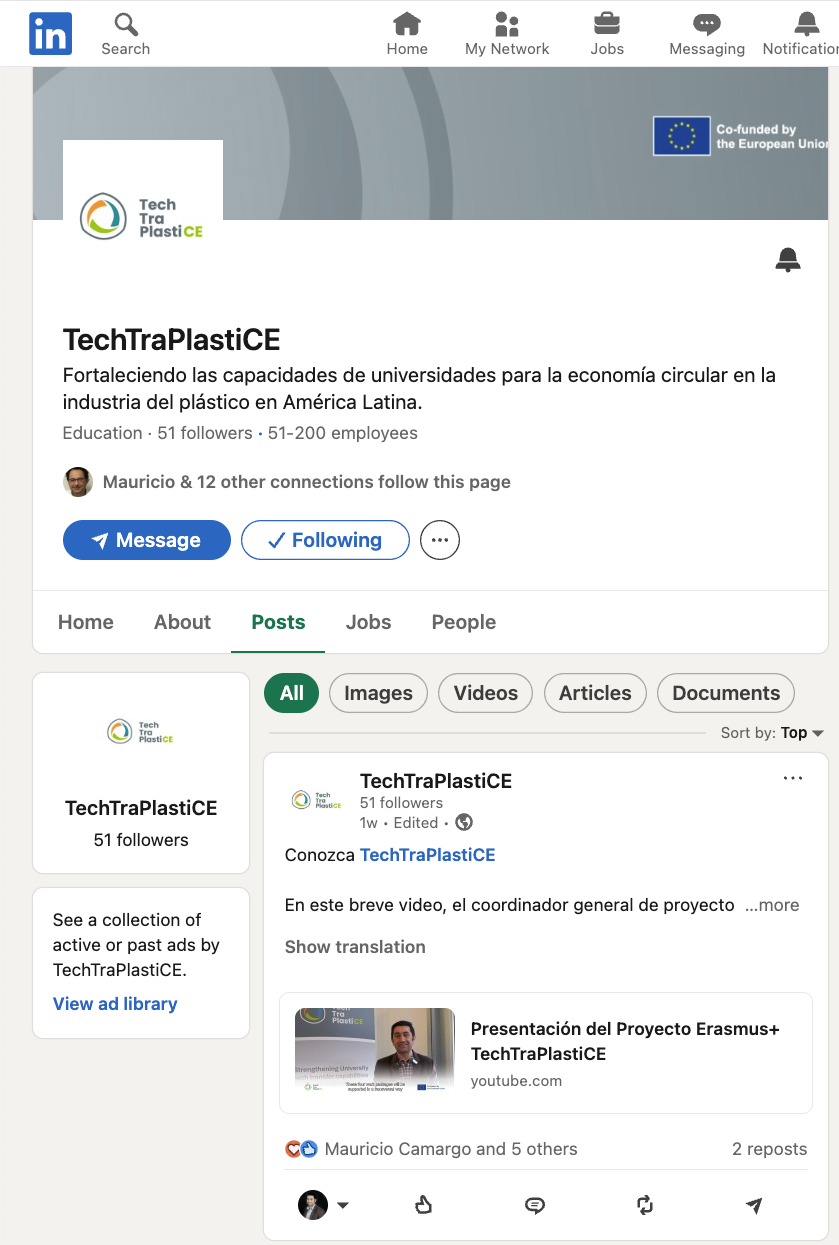
\includegraphics[width=0.6\linewidth,height=\textheight,keepaspectratio]{figures/5.3/linkedin.png}

}

\subcaption{\label{fig-linkedin}\href{https://www.linkedin.com/company/techtraplastice/}{LinkedIn}}

\end{minipage}%
%
\begin{minipage}[t]{0.02\linewidth}
~\end{minipage}%
%
\begin{minipage}[t]{0.32\linewidth}

\centering{

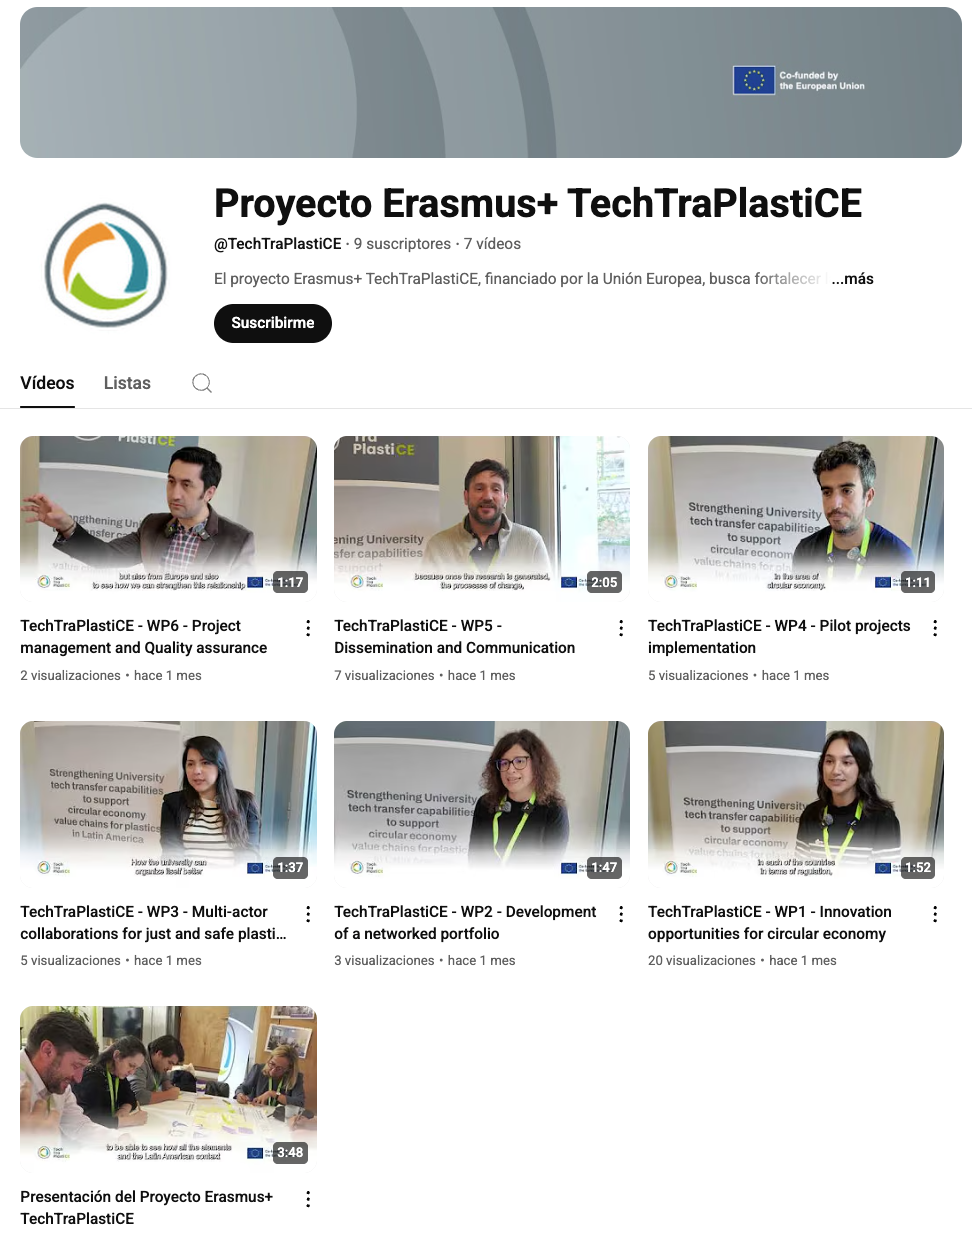
\includegraphics[width=0.6\linewidth,height=\textheight,keepaspectratio]{figures/5.3/youtube.png}

}

\subcaption{\label{fig-linkedin}\href{https://www.youtube.com/@TechTraPlastiCE}{Youtube}}

\end{minipage}%
%
\begin{minipage}[t]{0.02\linewidth}
~\end{minipage}%
%
\begin{minipage}[t]{0.32\linewidth}

\centering{

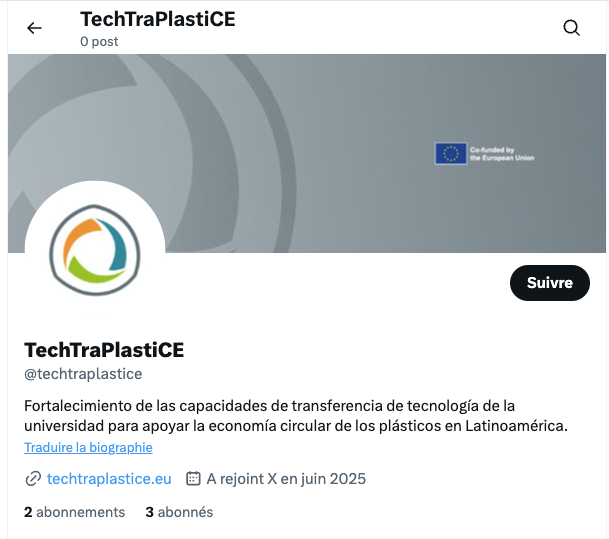
\includegraphics[width=0.6\linewidth,height=\textheight,keepaspectratio]{figures/5.3/X.png}

}

\subcaption{\label{fig-linkedin}\href{https://x.com/techtraplastice}{X}}

\end{minipage}%

\caption{\label{fig-social}Social accounts of TechTraPlastiCE project}

\end{figure}%

Partners have to follow the project's accounts, replicate the content
and comment to generate interaction.

The WP5, with the collaboration of all partners, will create content
considering other social media networks to be shared by the partners
through their institutional accounts, such as Instagram.

The linkedIn account was created on April 2025 and it count 51 followers
at the moment of writing this rapport. The main purpose with this
account is to connect with external socio-economic actor thanks to this
professional account channel.

The X account was created on 24 June 2025. The main purpose with this
account is to connect with a general audience that can be interested in
the topic of circular economy that eventually can pass to a professional
communication.

Finally, the YouTube Channel was created on May 19, 2025. At the moment
of writing this rapport, there are

\begin{itemize}
\tightlist
\item
  Subscribers: 9
\item
  Videos Published: 7
\item
  Views: 68
\end{itemize}

WP5 leader will map the audience indicators as a proxy of the impact of
the activities developed at TechTraPlastiCE project

\section{Social Media Content
Coordination}\label{social-media-content-coordination}

Social media channels play a complementary and amplifying role in the
overall dissemination strategy of TechTraPlastiCE. Their purpose is to
extend the visibility of the project's activities, connect with diverse
stakeholder communities, and drive traffic toward the official project
website, where detailed information and resources are hosted.

To ensure coherence and consistency across all communication platforms,
the WP5 leader coordinates the planning and publication of content on
\textbf{LinkedIn}, \textbf{X (formerly Twitter)}, and \textbf{YouTube},
with contributions from all partners.\\
Each partner is encouraged to share and repost TechTraPlastiCE content
through their institutional and professional networks, thereby enhancing
the project's outreach and engagement.

Social media content is prepared following a shared editorial calendar,
aligned with the monthly website update cycle (see Figure
Figure~\ref{fig-calendar}). This coordination guarantees that the
messaging remains timely, coherent, and aligned with project milestones
and events.

The types of content published on social media include:

\begin{itemize}
\tightlist
\item
  Announcements of \textbf{project events, workshops, and training
  activities}.
\item
  Highlights of \textbf{key deliverables and milestones}
\item
  \textbf{Partner achievements} and relevant collaborations.
\item
  \textbf{Multimedia content} (e.g., short videos, infographics, and
  visuals) to increase audience engagement.
\item
  Links to \textbf{news articles, publications, and website updates}.
\end{itemize}

All posts follow the project's visual identity and branding guidelines
(as defined in D5.2 -- Branding Toolkit and Training Plan) and adhere to
the principles of clarity, accessibility, and professionalism expected
in European projects.

\chapter{Conclusions}\label{conclusions}

The TechTraPlastiCE website and its associated digital channels
successfully fulfill their primary goal of supporting communication,
visibility, and knowledge sharing across all stages of the project.
Designed under the coordination of WP5 by Universidad Nacional de Río
Negro, and with the collaboration of all partners, the platform is more
than an information repository---it functions as the central hub for
dissemination and engagement. With its clean layout, multilingual
accessibility, and structured sections (Home, Project, Partners, News,
Agenda, and Contact), it provides targeted content to diverse audiences,
from academic stakeholders to enterprises and the general public.

The integration of news, events, and contact forms ensures up-to-date
information and two-way communication. Social media accounts on
LinkedIn, X, and YouTube serve to amplify the project's impact by
extending its reach beyond institutional circles. These channels help
redirect audiences to the official website while also offering
additional formats to share research outputs and project milestones.

While the current platform offers strong foundations in terms of
functionality and coherence, it also presents opportunities for growth
in terms of visual engagement and user interaction. As noted, there is
room to enhance the Project section through the inclusion of
infographics and visual storytelling elements that better explain
complex ideas to non-technical users. Future development stages could
also improve mobile optimization---particularly for the news
section---and expand the content diversity shared on partner and
institutional platforms. Moreover, the continued collaboration among
partners in content creation, guided by shared templates and editorial
calendars, will help maintain the website's relevance and visibility.
Regular updates and responsive design contribute to transparency and
traceability, while the inclusion of analytics from social platforms
will support performance tracking. In sum, the TechTraPlastiCE digital
strategy reflects a well-structured, scalable communication framework
aligned with European Commission expectations and the project's broader
objectives.

\appendix

\chapter{Templates for content generation}\label{sec-template}

A template was designed to all members in order to put news of
techtraplastice website.

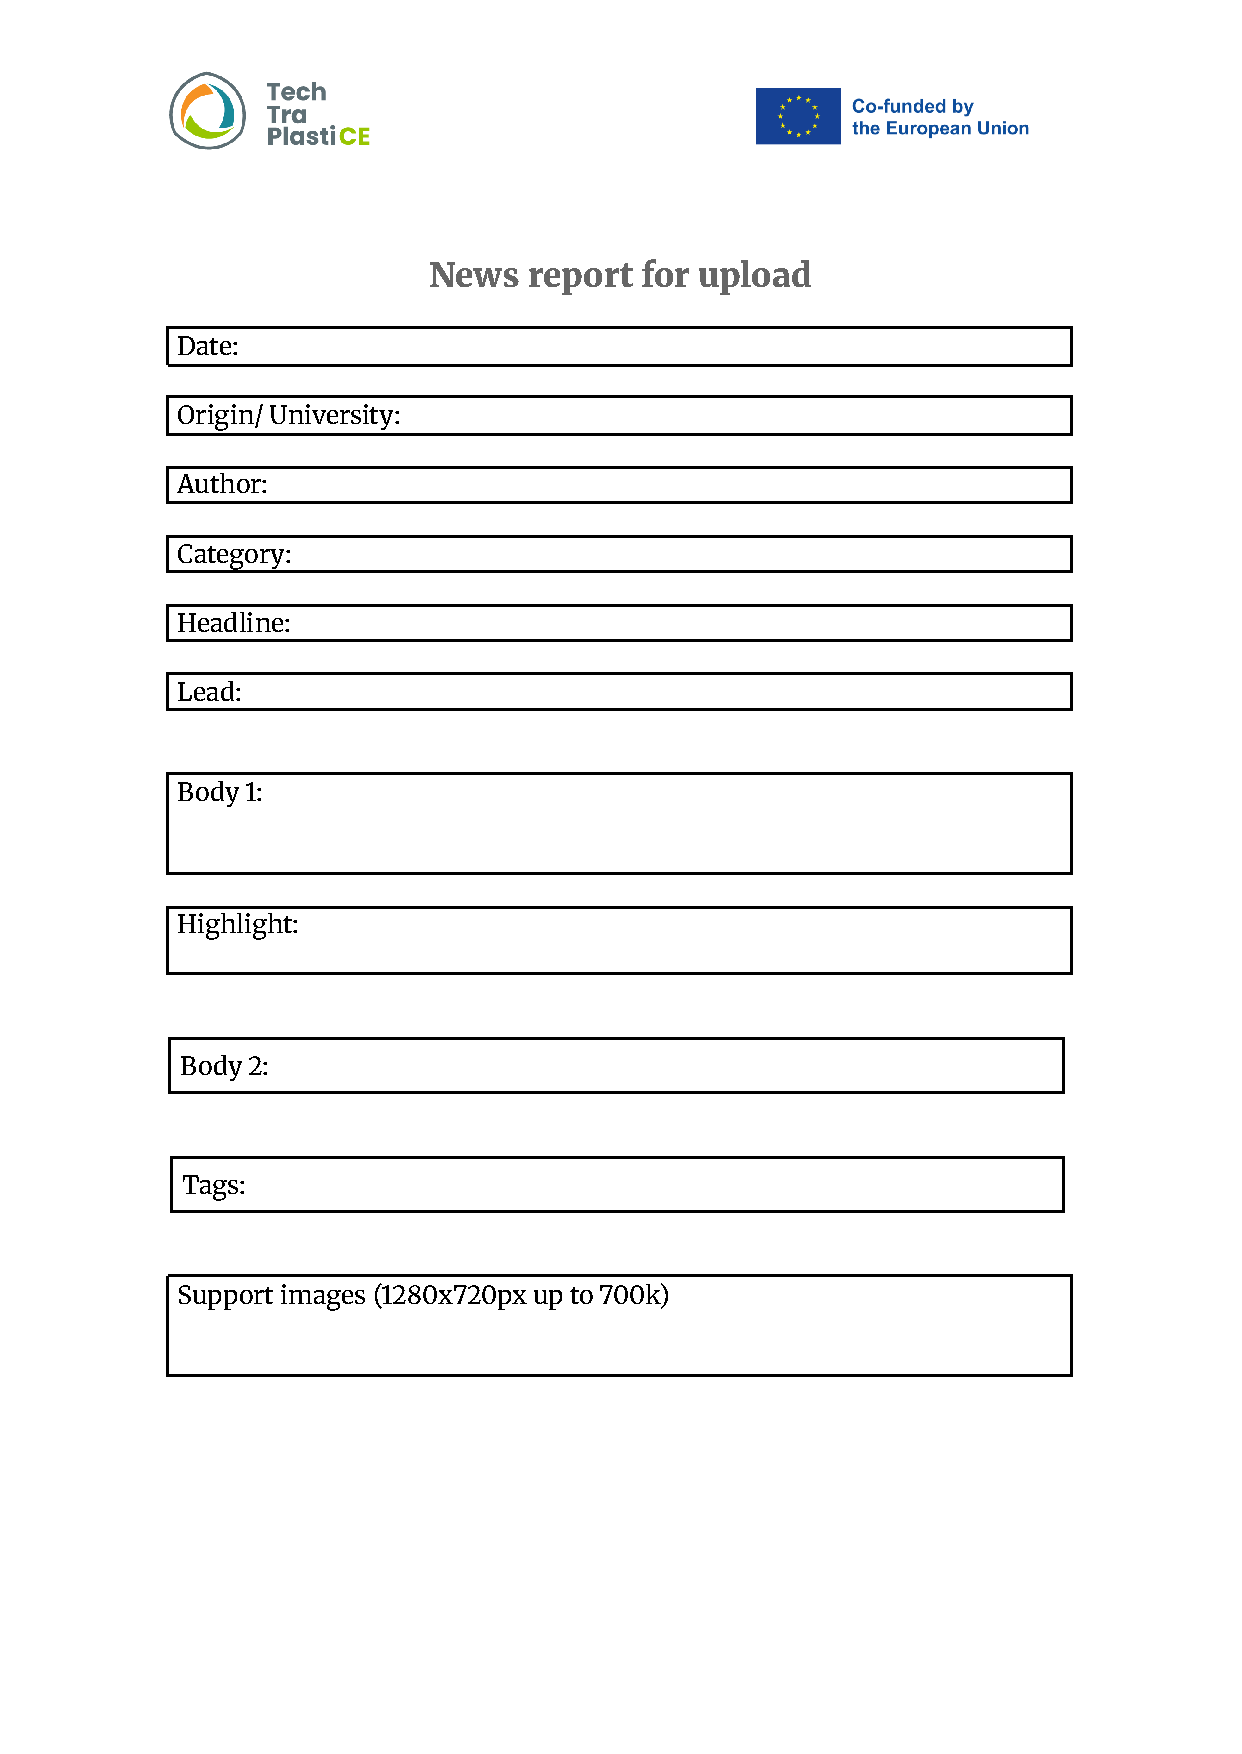
\includepdf[scale=0.8, 
pagecommand={\pagestyle{fancy}}, frame=true, pages=-]{figures/5.3/Template.pdf}


\backmatter


\end{document}
